\documentclass[Nike]{tuberlinbeamer}

\usepackage{dsfont}

%\usepackage[ngerman]{babel}  % 'babel' muss geladen werden
\usepackage[utf8]{inputenc}  % optional, aber empfehlenswert
\usepackage[square,numbers]{natbib}
\usepackage{bibentry}



\usepackage[]{algorithm2e}
\usepackage{caption}
\captionsetup[figure]{labelformat=empty}
\usepackage[ddmmyyyy]{datetime}
\usepackage{subcaption}



% Die ueblichen Angaben
\title{Designing Recurrent Neural Networks for Explainability
}
%\subtitle{\today}
\author[Pattarawat Chormai  $\mid$ \today]{Pattarawat Chormai}
\institute{Master's thesis supervised by Prof. Klaus-Robert M\"{u}ller \& Dr. Gr\'{e}goire Montavon}

% Eigenes Logo einfuegen:
\renewcommand{\pathtomylogo}{}
\newcommand{\x}[0]{\boldsymbol{x}}
\newcommand{\pvec}[1]{\boldsymbol{#1}}
\newcommand{\ppartial}[2]{\frac{\partial #1}{\partial #2}}
\renewcommand{\pagename}{Page} 



\begin{document}

\begin{frame}
\maketitle
\end{frame}


%\begin{frame}{Outline}
%\tableofcontents
%\end{frame}


%\section{Objective}	
\begin{frame}{Motivation}

\begin{itemize}
	\item Impact of the architecture of RNNs on explainability
	\item Do deep RNNs have more explainable predictions? 
	\item Are there ways to make RNNs more explainable?
\end{itemize}
\end{frame}

\begin{frame}{Recurrent Neural Networks (RNNs)}

	\begin{itemize}
		\item \textbf{Successful applications:} \\ $\rhd$ machine translation \citep{DBLP:journals/corr/WuSCLNMKCGMKSJL16}, image captioning \citep{DBLP:conf/cvpr/VinyalsTBE15,DBLP:conf/nips/VaswaniSPUJGKP17}
	\end{itemize}
	\begin{figure}[h]
		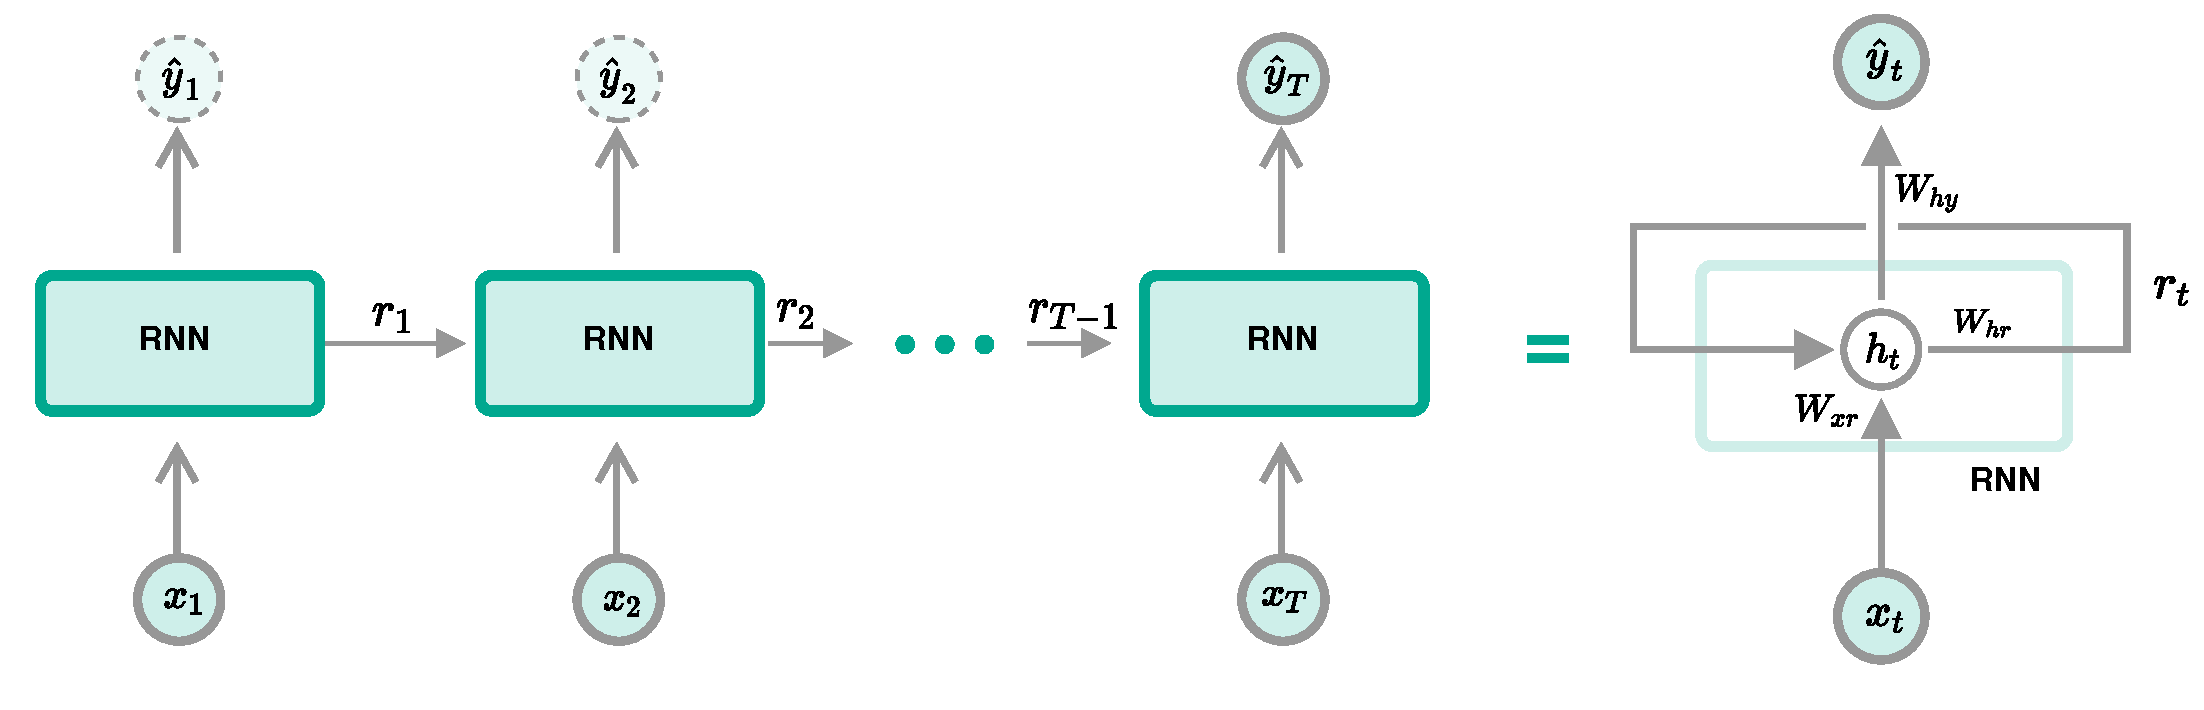
\includegraphics [width=\textwidth]{figures/present_rnn_unfold_1}
	\end{figure}
 	
\end{frame}

\begin{frame}{Explainability}
\begin{itemize}
	\item Ability to provide \textbf{sensible explanation} towards how input associates to a certain prediction
	\item \textbf{Analogy:} why does the RNN classify this text as a positive review?

	\begin{figure}[h]
		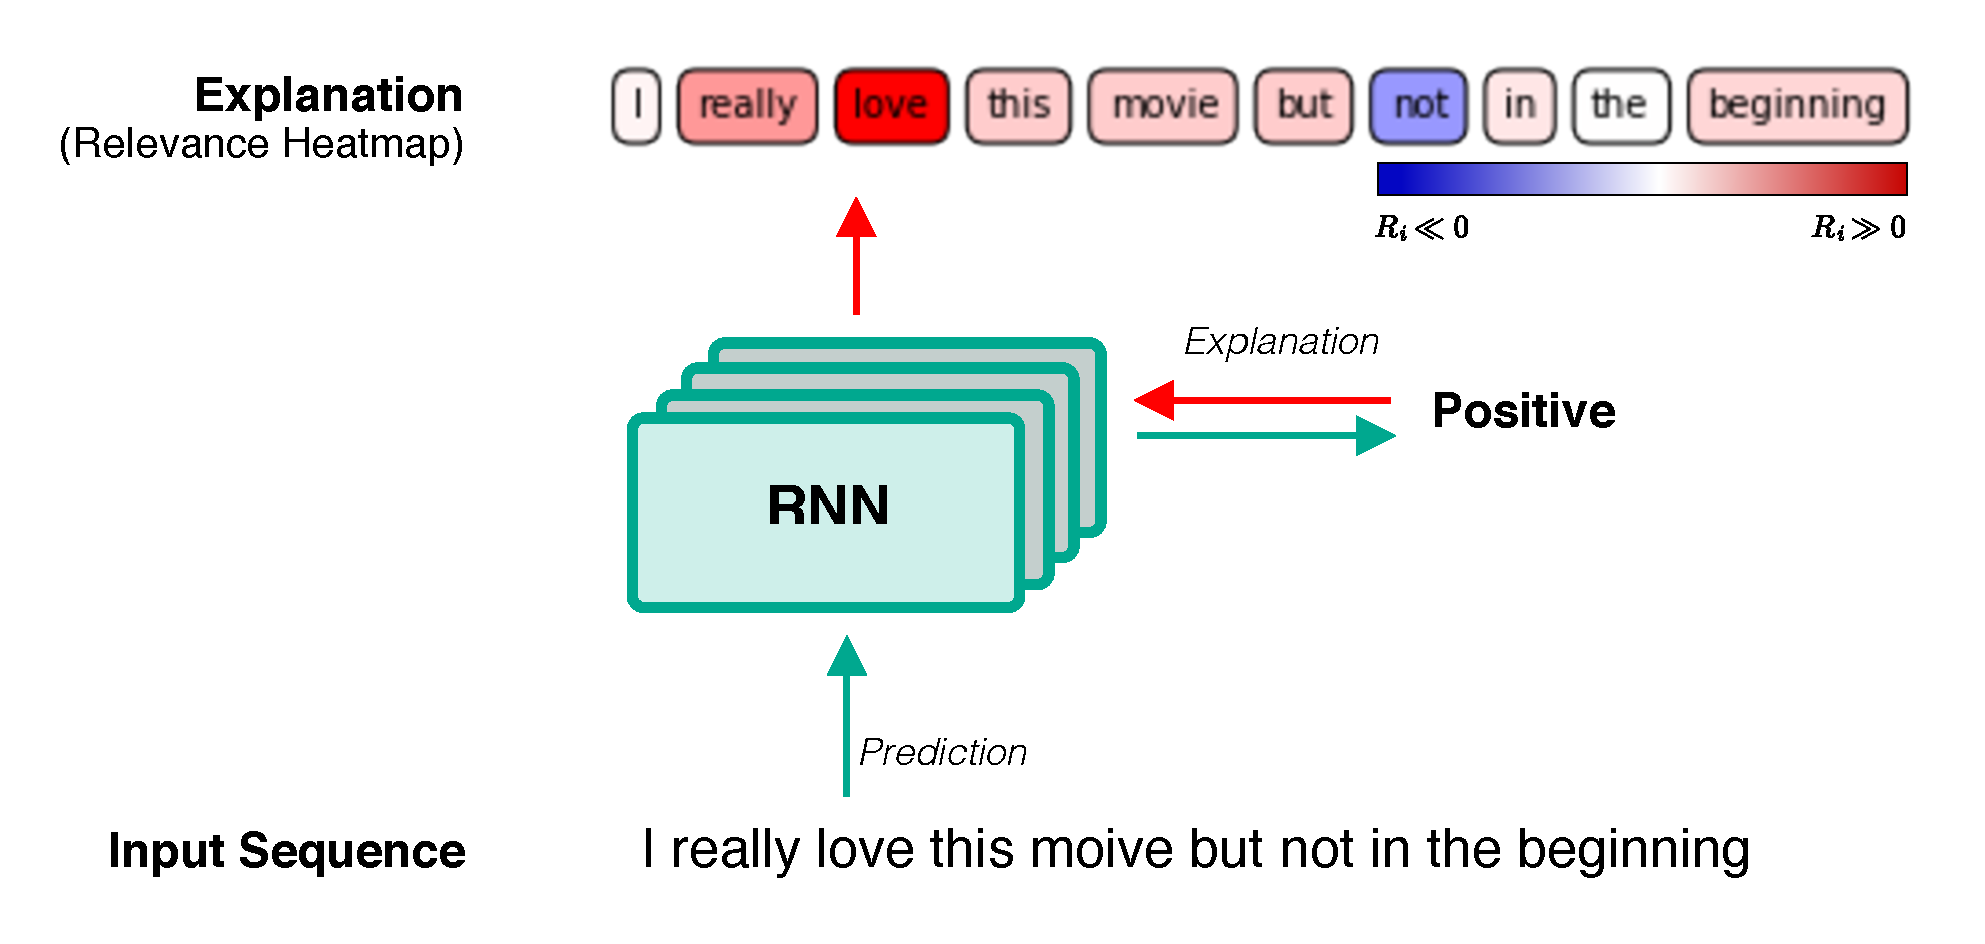
\includegraphics [width=0.8\textwidth]{figures/present_explanation_rnn}
	\end{figure}
	
%	\item Why do we need explainable models?\begin{itemize}
%		\item Aid decision and establish trust in the system, especially in critical applications such as healthcare.
%	\begin{figure}[h]
%		\centering
%%		\begin{subfigure}[b]{0.45\linewidth}
%%		  \centering
%%
%%			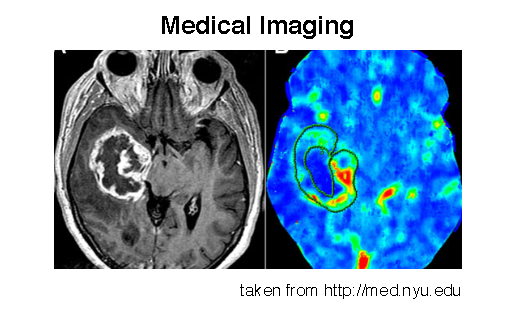
\includegraphics [width=0.9\textwidth]{figures/present_medical_imaging_cnn}
%%		\end{subfigure}
%		\begin{subfigure}[b]{0.5\linewidth}
%		  \centering
%
%			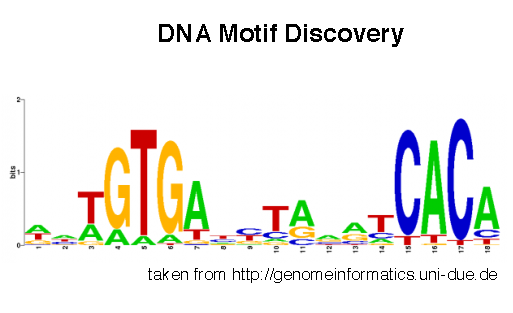
\includegraphics [width=0.9\textwidth]{figures/present_motif_discovery}
%		\end{subfigure}
%	\end{figure}
%		\item Developers can assure that trained models would work as expected.
%		\end{itemize}
\end{itemize}
	
\end{frame}



\section{Explanation Methods}
\begin{frame}[allowframebreaks=0.95,t]{Explanation Methods}

\begin{enumerate}
	\item Sensitivity Analysis \citep{SimonyanDeepConvolutionalNetworks2013} (SA)
			\begin{align*}
				R_i(\x) = \bigg ( \ppartial{f(\x)}{x_i} \bigg )^2
			\end{align*}
	\item Guided Backprop \citep{SpringenbergStrivingSimplicityAll2015a} (GB) \\
		\begin{itemize}
			\item Developed for explaining \textbf{ReLU}-based CNNs
		\end{itemize}
				\begin{align*}
				\frac{\partial_{*} f(\x) }{\partial h_j} = \mathds{1} \bigg[  h_j > 0 \bigg]\max\bigg( 0, \frac{\partial_{*} f(\x) }{\partial a_j} \bigg);\hspace{1cm} R_i(\x) = \bigg( \frac{\partial_{*} f(\x) }{\partial x_i} \bigg )^2
%				R_i(\x) = \bigg ( \frac{\partial #1}{\partial #2}\ppartial{f(\x)}{\x} \bigg )^2
			\end{align*}
	\framebreak
	
	\item Layer-wise Relevance Propagation \citep{BinderLayerWiseRelevancePropagation2016}  (LRP) 
		\begin{itemize}
			\item Distributing relevance based on \textbf{neurons' activities}
			\begin{columns}
			\column{0.5\textwidth}{
				\begin{figure}[h]
					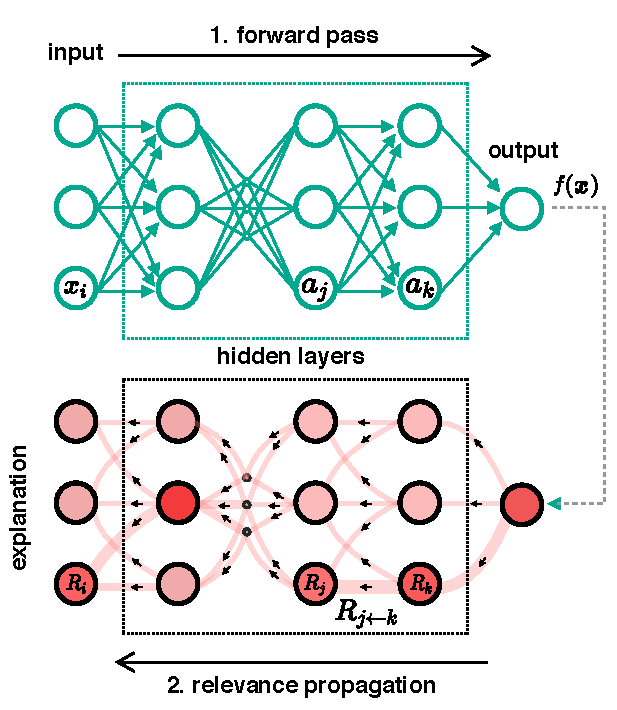
\includegraphics [width=0.75\textwidth]{figures/present_lrp_graph}
				\end{figure}

			}
			\column{0.5\textwidth}{
			   \vspace{1.5cm}\\
			LRP-$\alpha\beta$ rule:
			\begin{align*}
				R_j(\x) = \sum_k \bigg( \alpha \frac{a_j w_{jk}^+}{\sum_{j'} a_{j'} w_{j'k}^+}  - \beta  \frac{a_j w_{jk}^-}{\sum_{j'} a_{j'} w_{j'k}^-}  \bigg) R_k(\x)
			\end{align*}
			}
		\end{columns}

		\end{itemize}
	\vspace{3cm}
	
	 \item Deep Taylor Decomposition  \citep{MontavonExplainingnonlinearclassification2017} (DTD)
		\begin{itemize}
			\item LRP's theoretical view for explaining \textbf{ReLU-based} architectures
			\begin{align*}
				R_k = R_k \bigg|_{\{ \tilde{a}_j \}_j} + \sum_j \frac{\partial R_k}{\partial a_j} \bigg|_{\{ \tilde{a}_j \}_j} (a_j - \tilde{a}_j ) + \xi_k \tag{Taylor expansion}
			\end{align*}
			\item Two important propagation rules:  \\
			-- $z^+$ for $a_j \in \mathbb{R}^+$ (LRP-${\alpha_{1}\beta_{0}}$)
			\begin{align*} 
				R_j  = \sum_k \frac{a_j w_{jk}^+ }{\sum_j a_j w_{jk}^+ }R_k 
			\end{align*}
			-- $z^\mathcal{B}$ for $a_j \in [l_j, h_j]$ where $l_j \le 0 < h_j$
			\begin{align*}
								R_j = \sum_k \frac{a_j w_{jk} - l_j w_{jk}^+ - h_j w_{jk}^- }{\sum_{j'} a_{j'} w_{j'k} - l_{j'} w_{j'k}^+ - h_{j'} w_{j'k}^- } R_k
			\end{align*}
		\end{itemize}
\end{enumerate}	
\end{frame}

%\begin{frame}{Example of relevance heatmaps}
%-- Explaining the classification decisions of a LeNet-5 type network.
%				\begin{figure}[h]
%					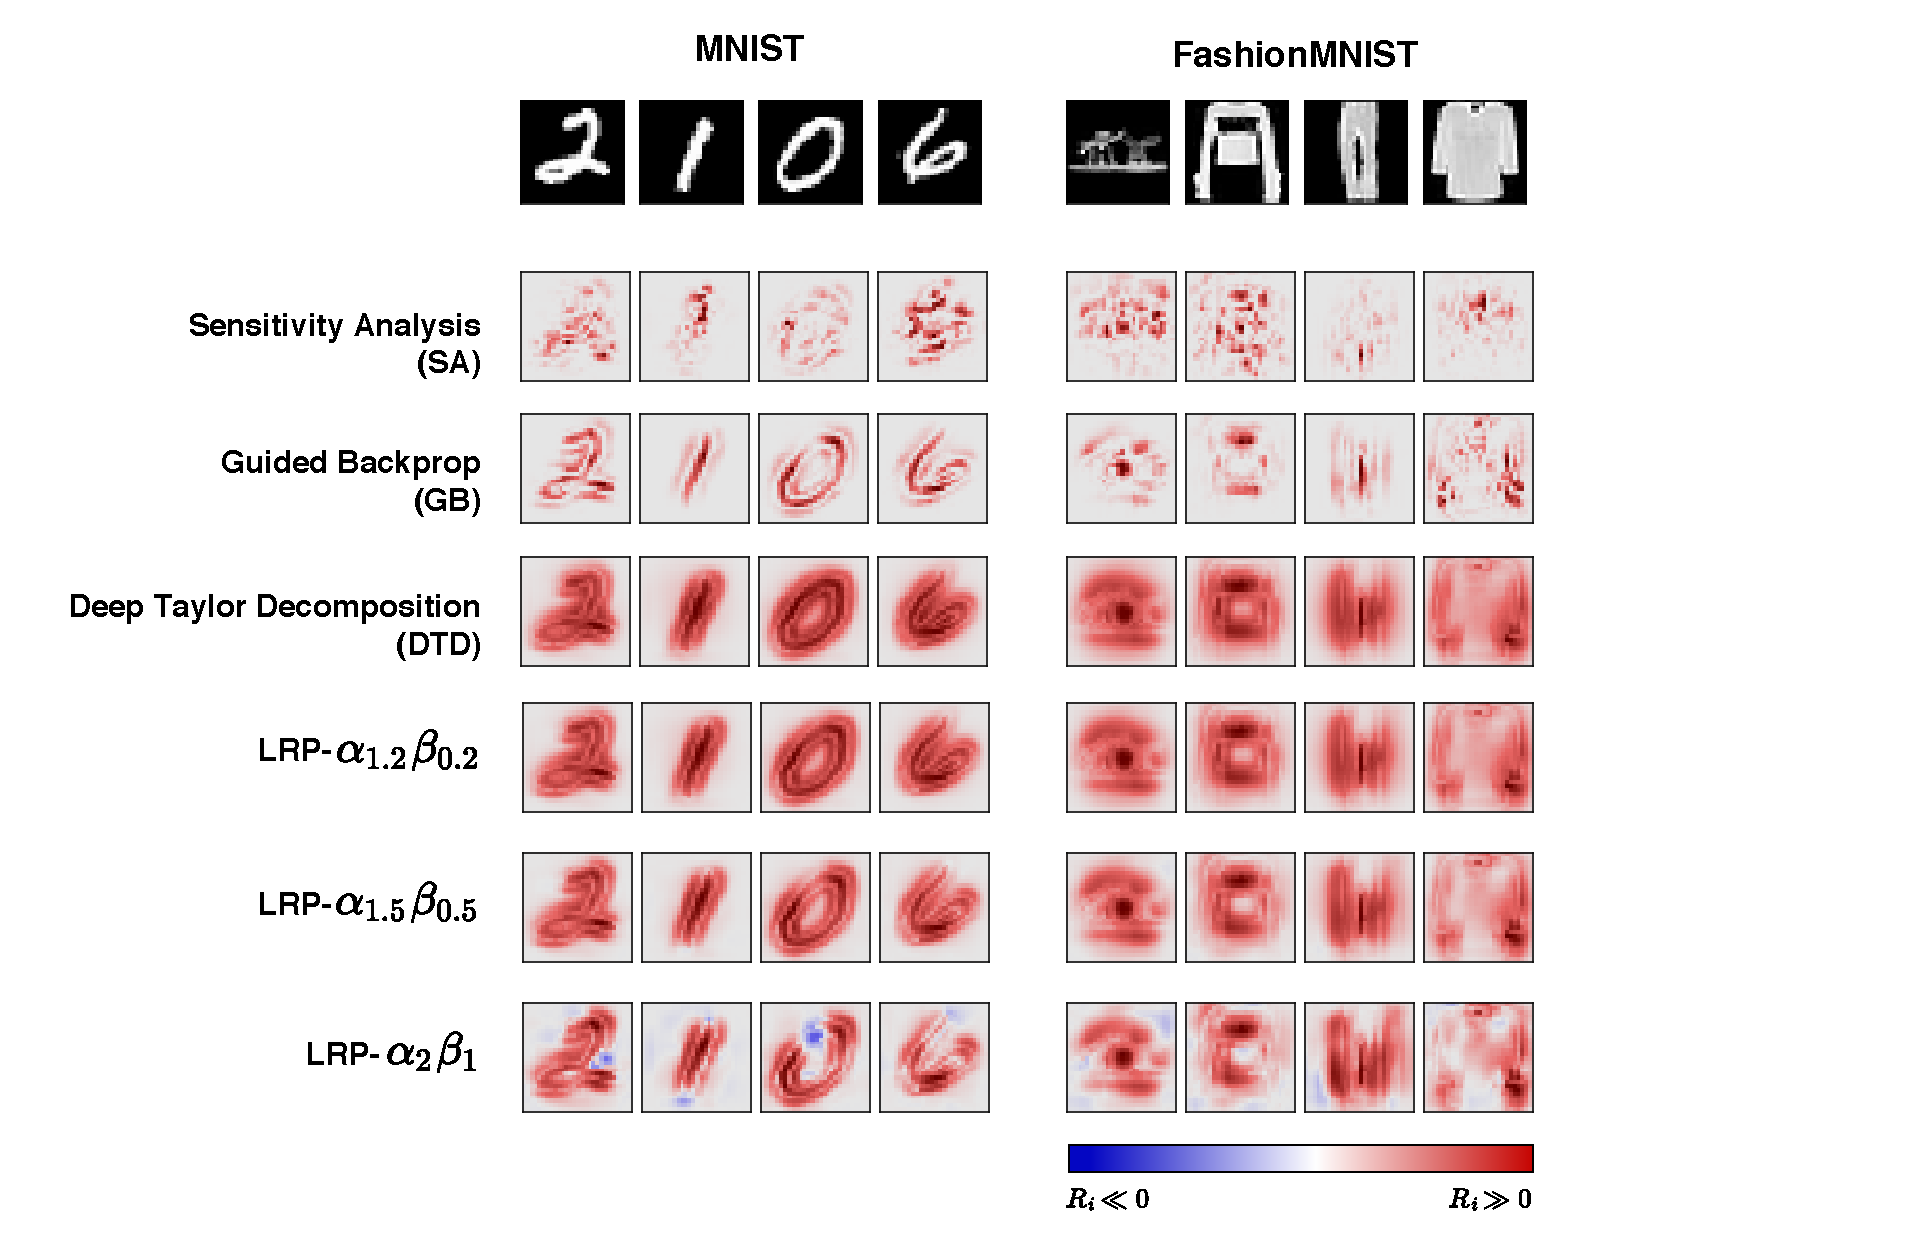
\includegraphics [width=0.7\textwidth]{figures/present_lenet_heatmaps}
%					\caption{ \tiny
%					Architecture: 
%								CONV(5$\times$5, 10) $\cdot$ AVGPOOL(2$\times$2, 2, 2) $\cdot$ 
%								CONV(5$\times$5, 25) $\cdot$ 
%								AVGPOOL(2$\times$2, 2, 2) $\cdot$
%								CONV(4$\times$4, 100)$\cdot$
%								AVGPOOL(2$\times$2, 2, 2) $\cdot$
%								DENSE(100) $\cdot$ DENSE(10)
%					}
%				\end{figure}
%
%%	 -  -  - AVG_POOL(2x2, 2, 2) - CONV(4x4, 100) - AVG_POOL(2x2, 2, 2)  - Dense(100) - DENSE (10)
%\end{frame}

\begin{frame}{Experimental Setup}
\begin{itemize}
	\item <1-2> \textbf{Problem:} Majority-Sample Sequence Classification (MNIST-MAJ, FashionMNIST-MAJ)
\only<1>{
	\newline
	$\rhd$ Sequence length: \textbf{12} \big($\{\x_t \in \mathbb{R}^{28\times7} \}_{t=1}^{12}$ \big) \\
	$\rhd$ Minimum accuracy 98\% for MNIST-MAJ and 89\% for FashionMNIST-MAJ


 \begin{figure}[h]
	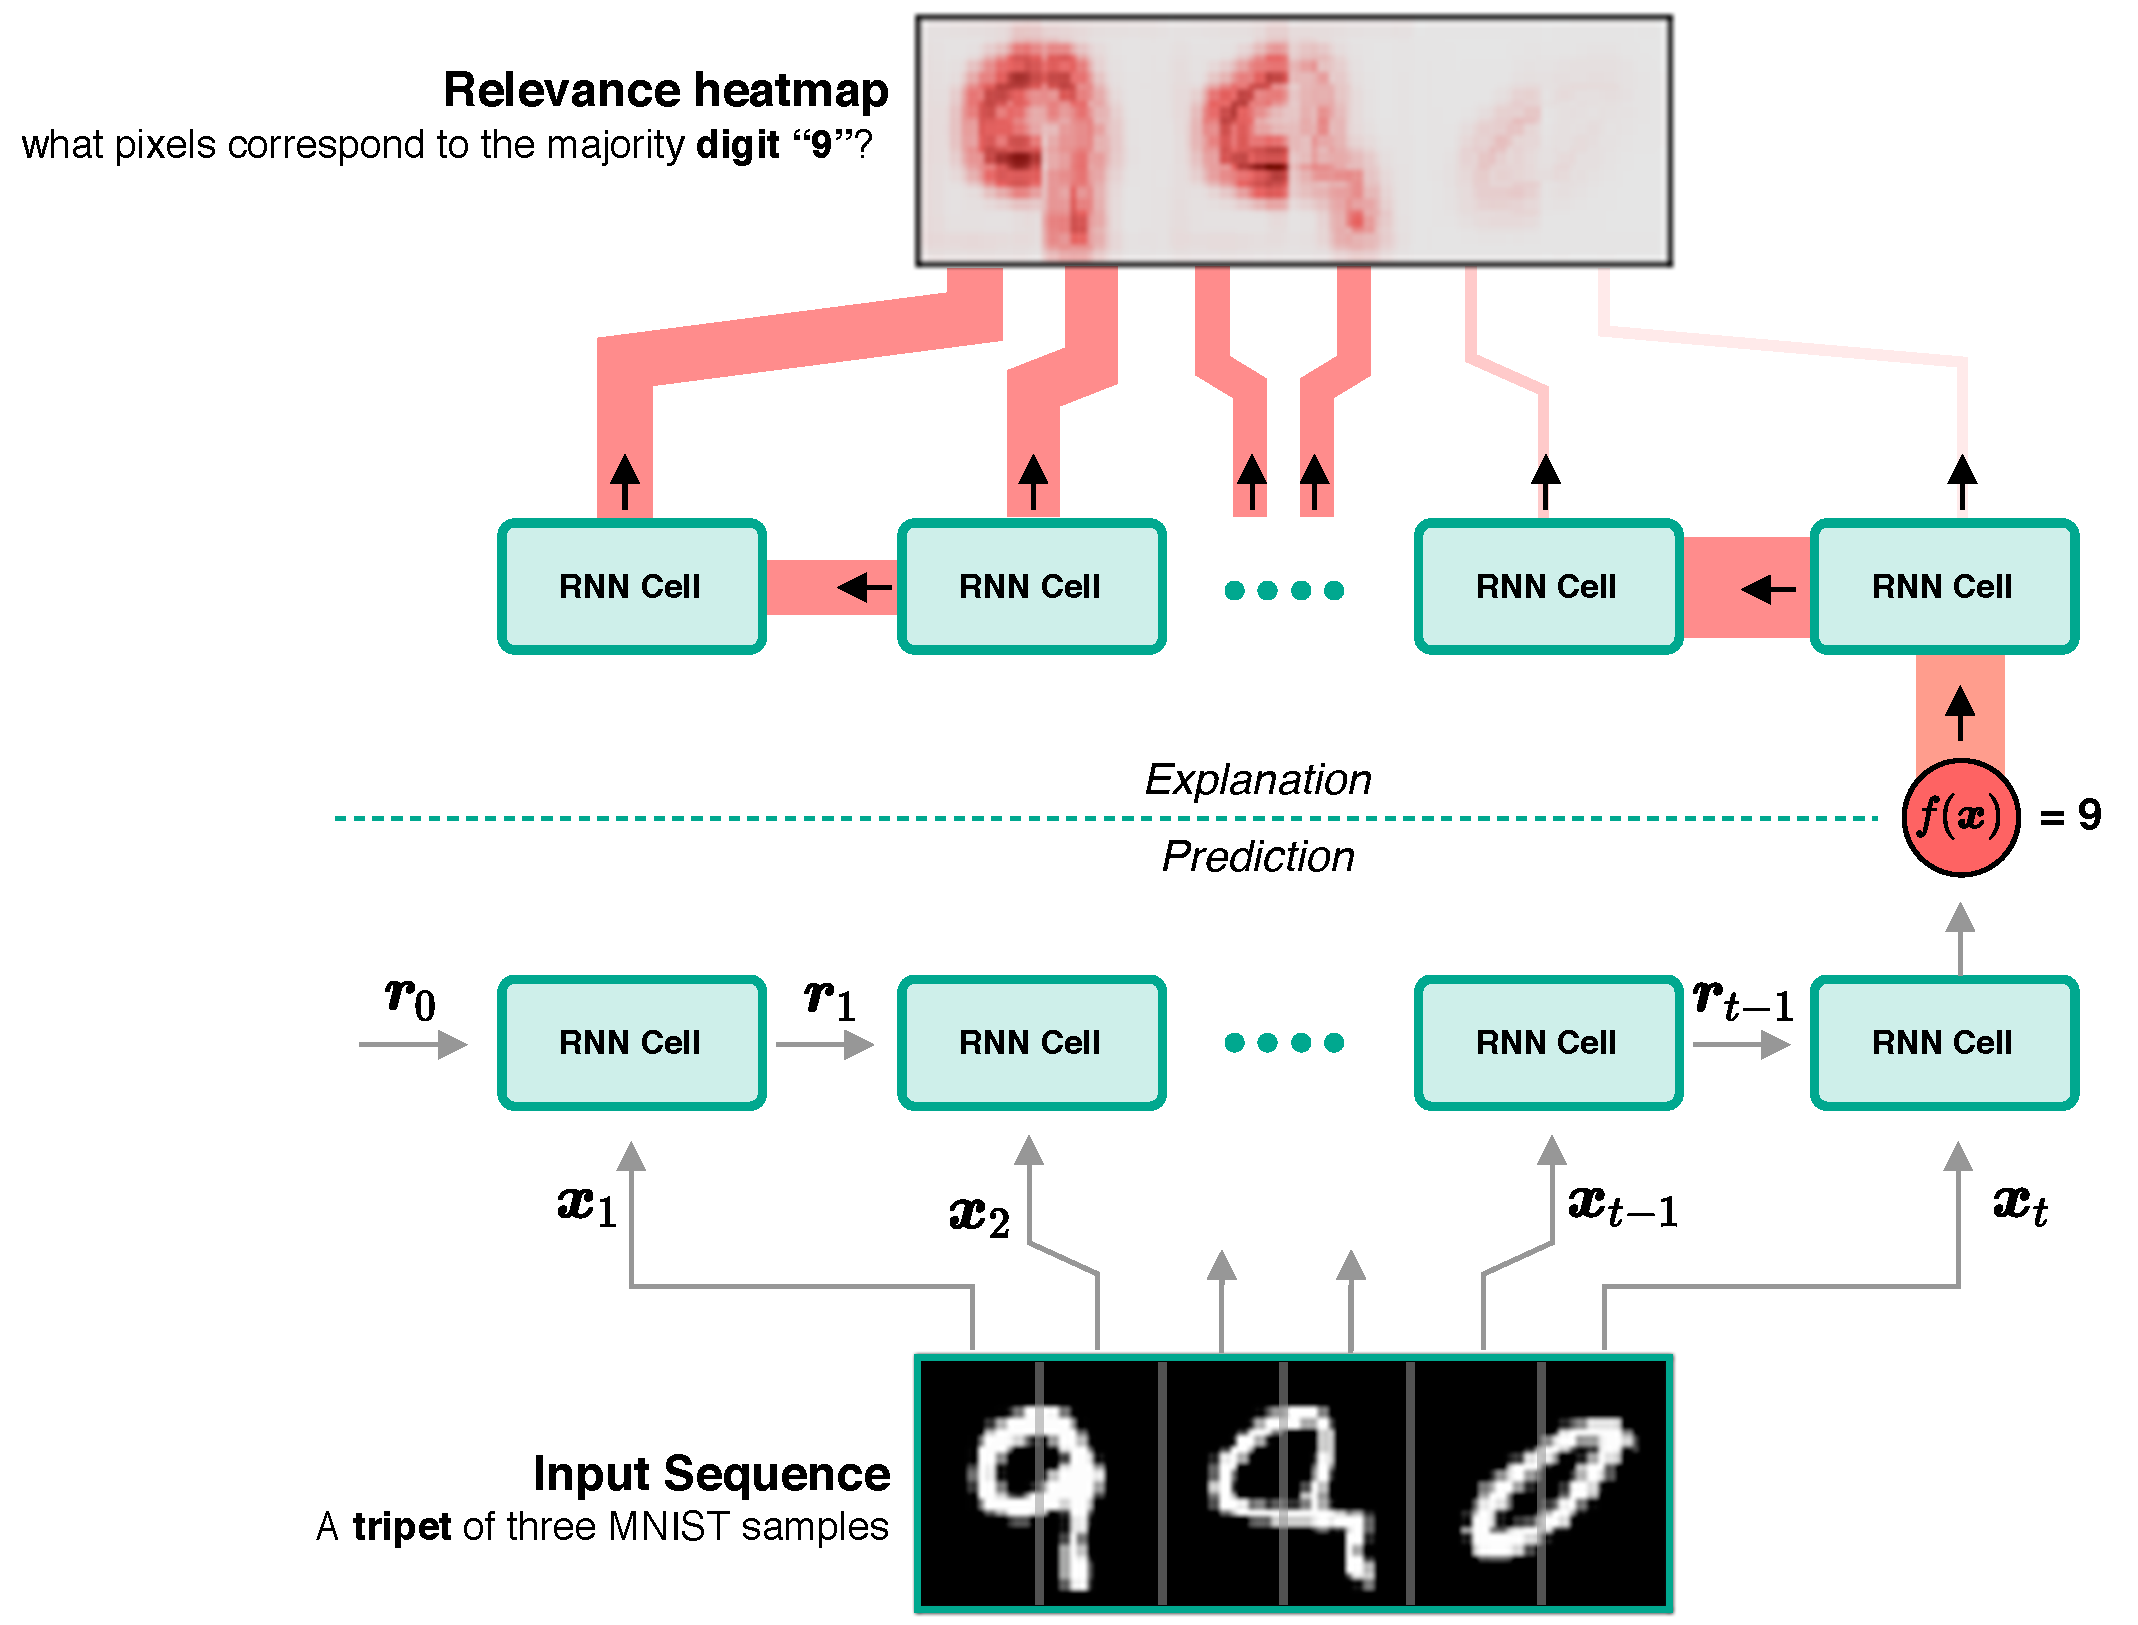
\includegraphics [width=0.55\textwidth]{figures/present_setting_2}
\end{figure}
}
\item <2> \textbf{Evaluation:} Cosine similarity (averaged over test samples)
 \begin{figure}[h]
	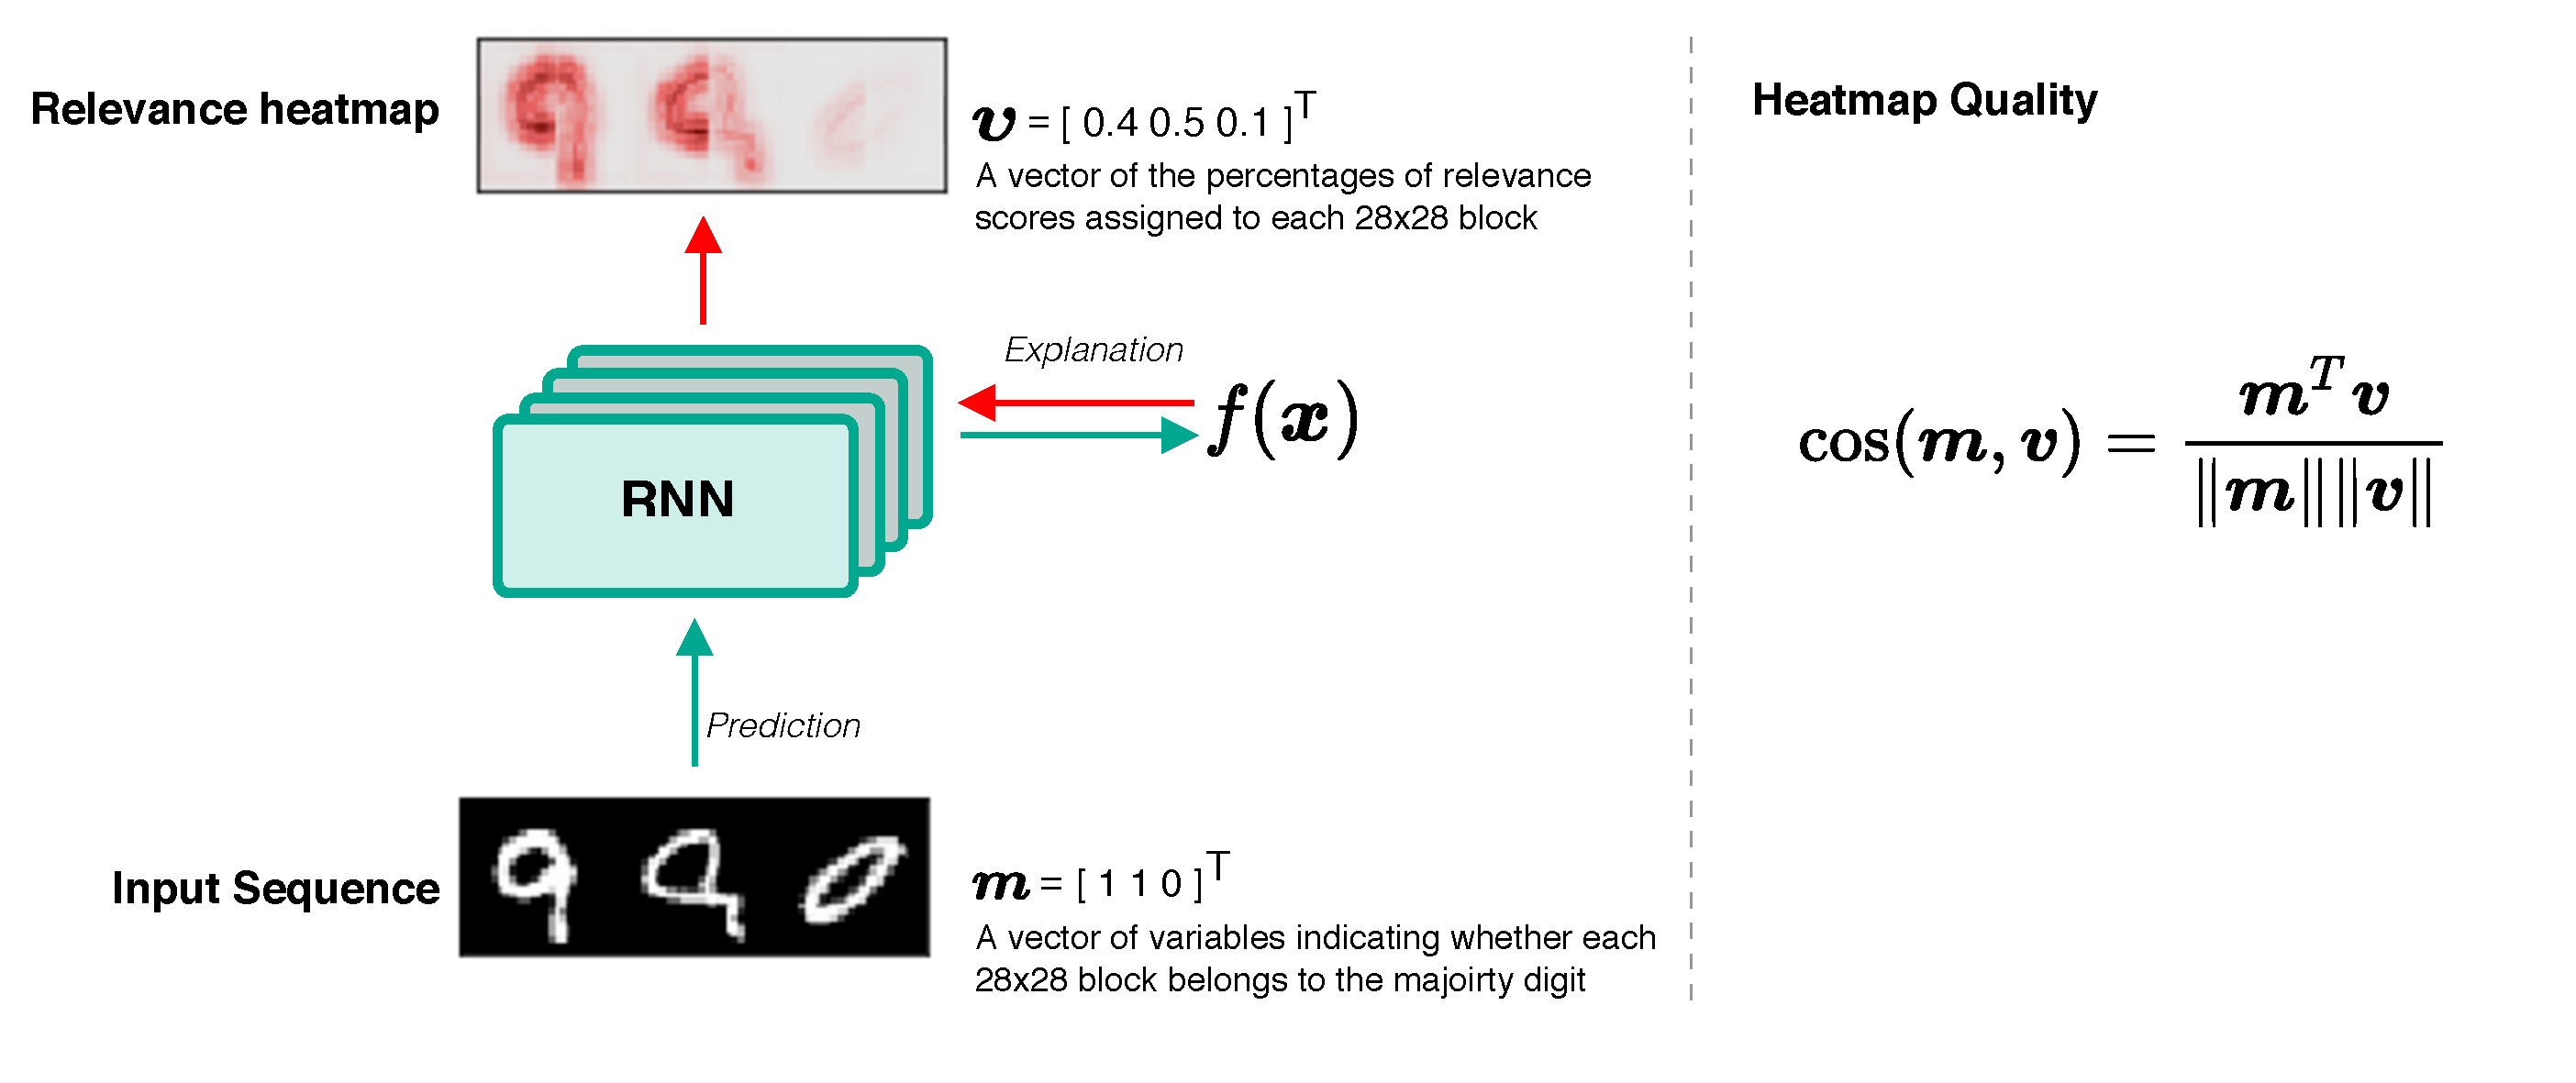
\includegraphics [width=0.85\textwidth]{figures/present_evaluation}
\end{figure}

\end{itemize}


\end{frame}

\begin{frame}{Experiment 1: Standard RNN Architectures}
\only<1>{

\vfill
 \begin{figure}[h]
	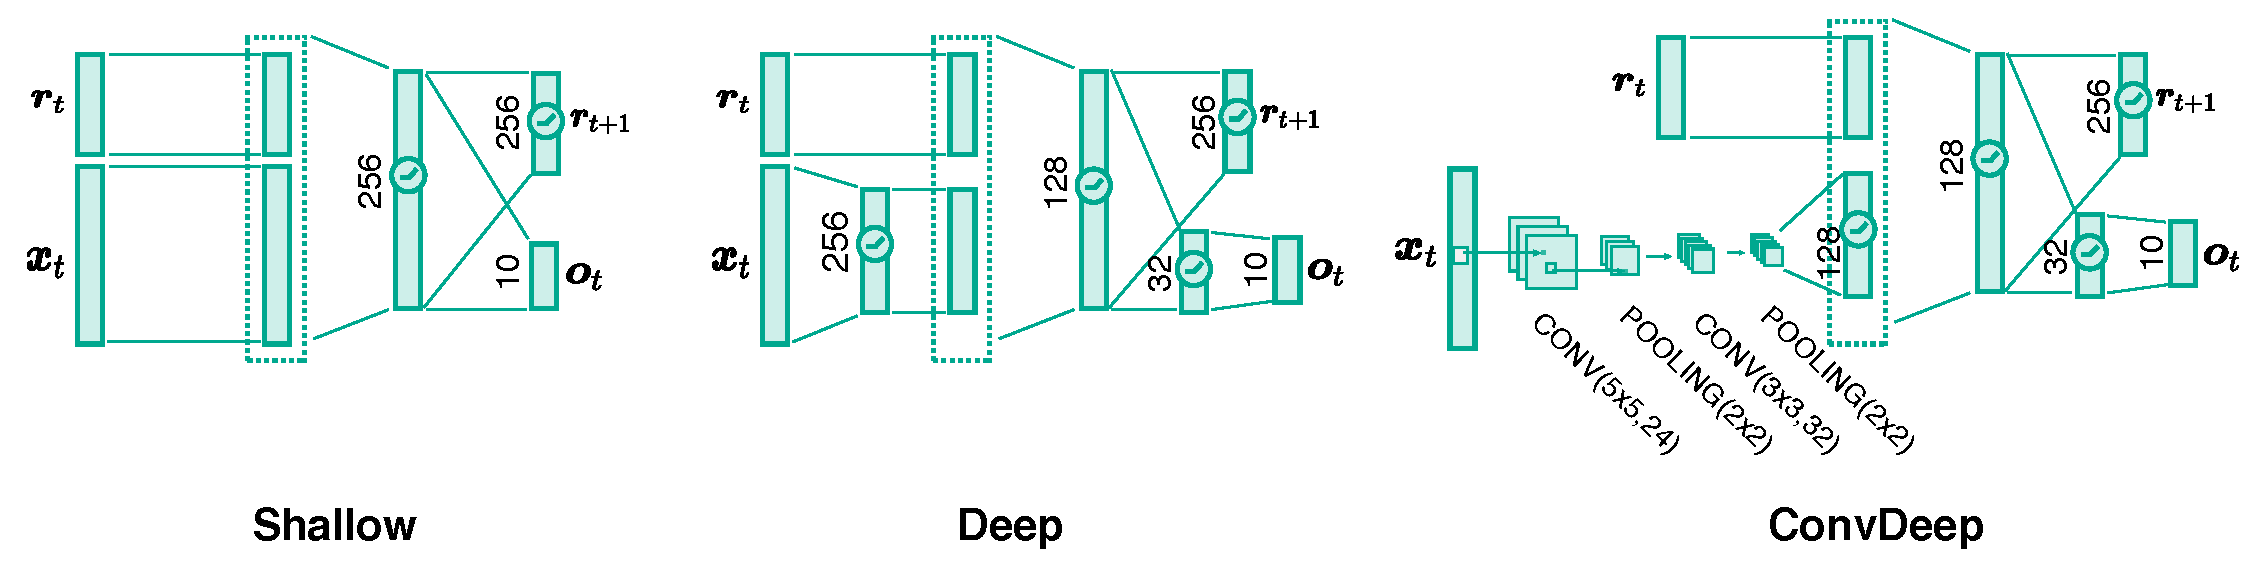
\includegraphics [width=\textwidth]{figures/present_exp1_standard_RNNs}
\end{figure}
\vfill
}
\only<2>{
Sample Relevance Heatmaps
\vfill
 \begin{figure}[h]
	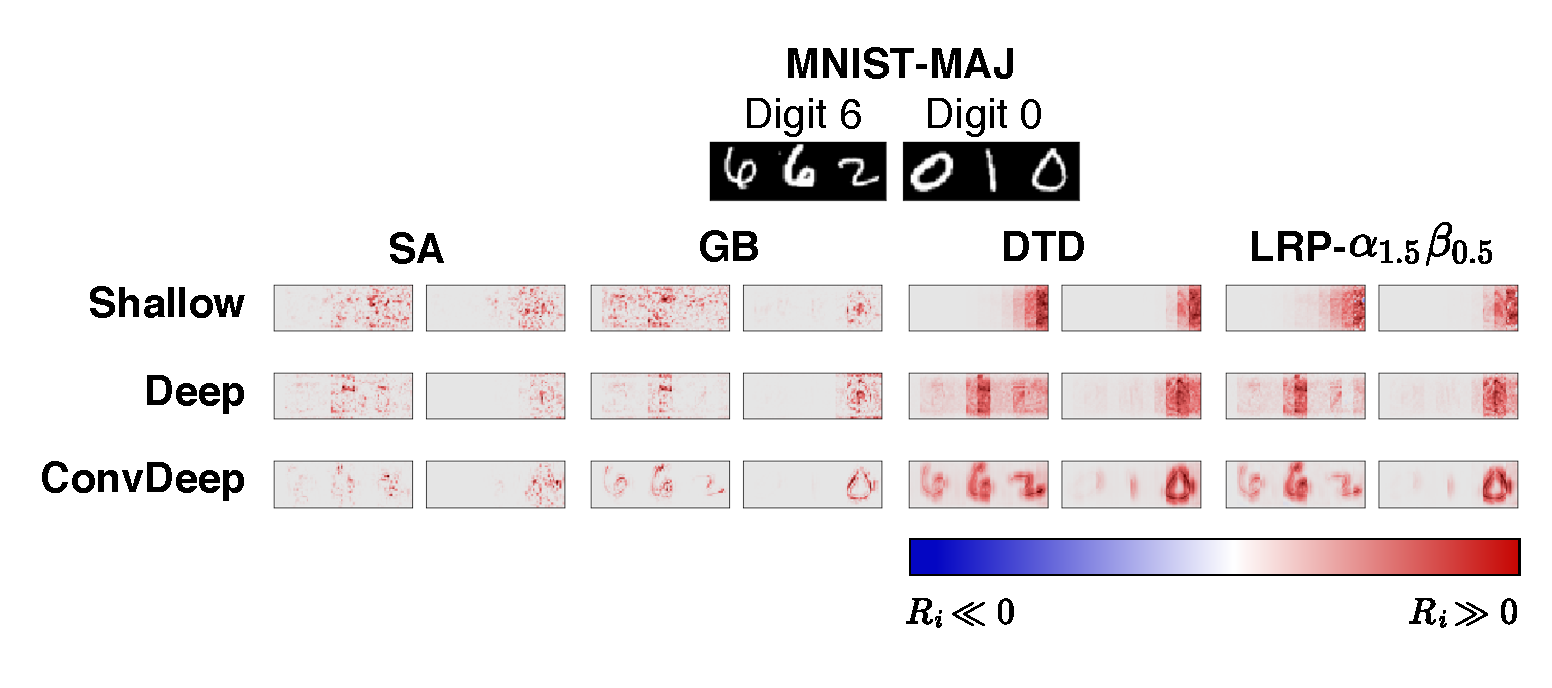
\includegraphics [width=0.8\textwidth]{figures/present_exp1_result_heatmap_only_mnist}
\end{figure}
\vfill

}
\only<3>{
Sample Relevance Heatmaps
\vfill
 \begin{figure}[h]
	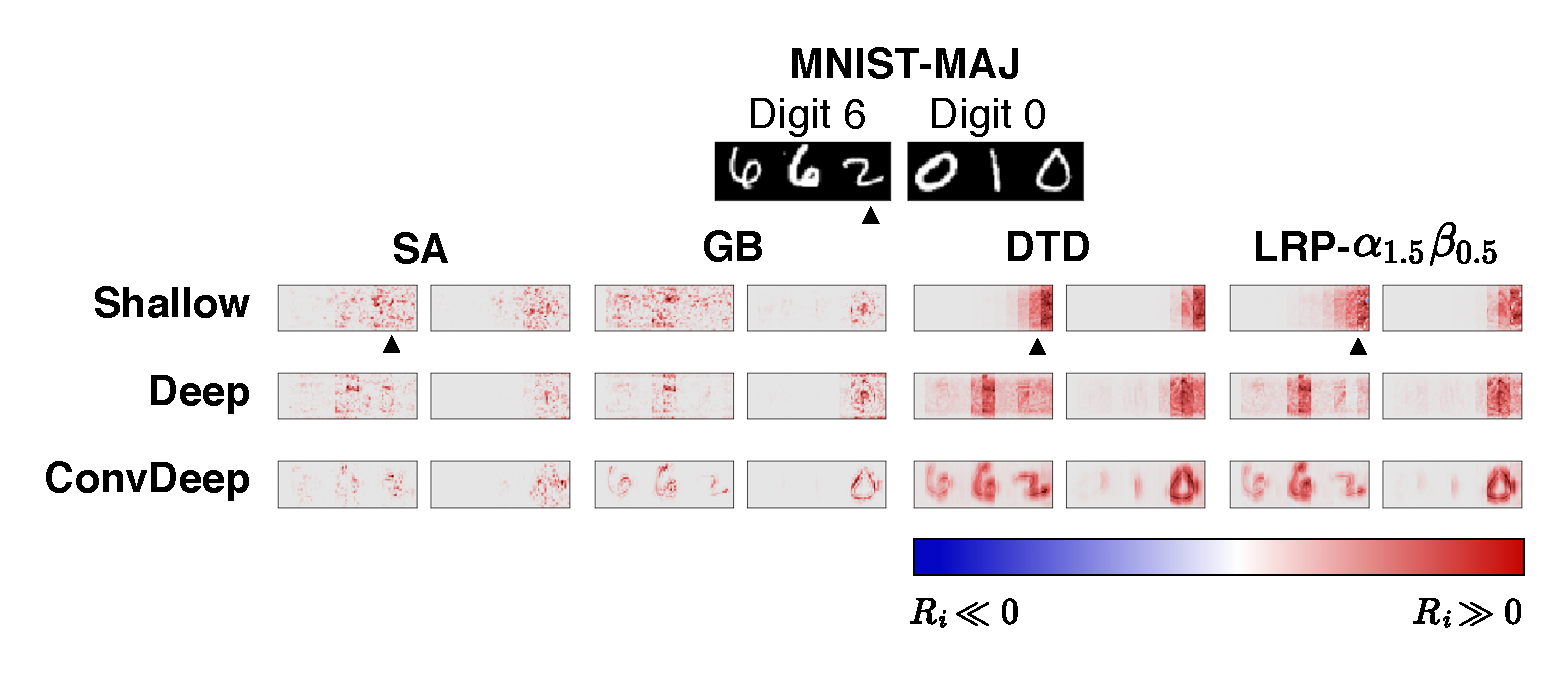
\includegraphics [width=0.8\textwidth]{figures/present_exp1_result_heatmap_2_only_mnist}
\end{figure}
\vfill

}



\only<4>{
Cosine Similarity Evaluation
\vfill
 \begin{figure}[h]
	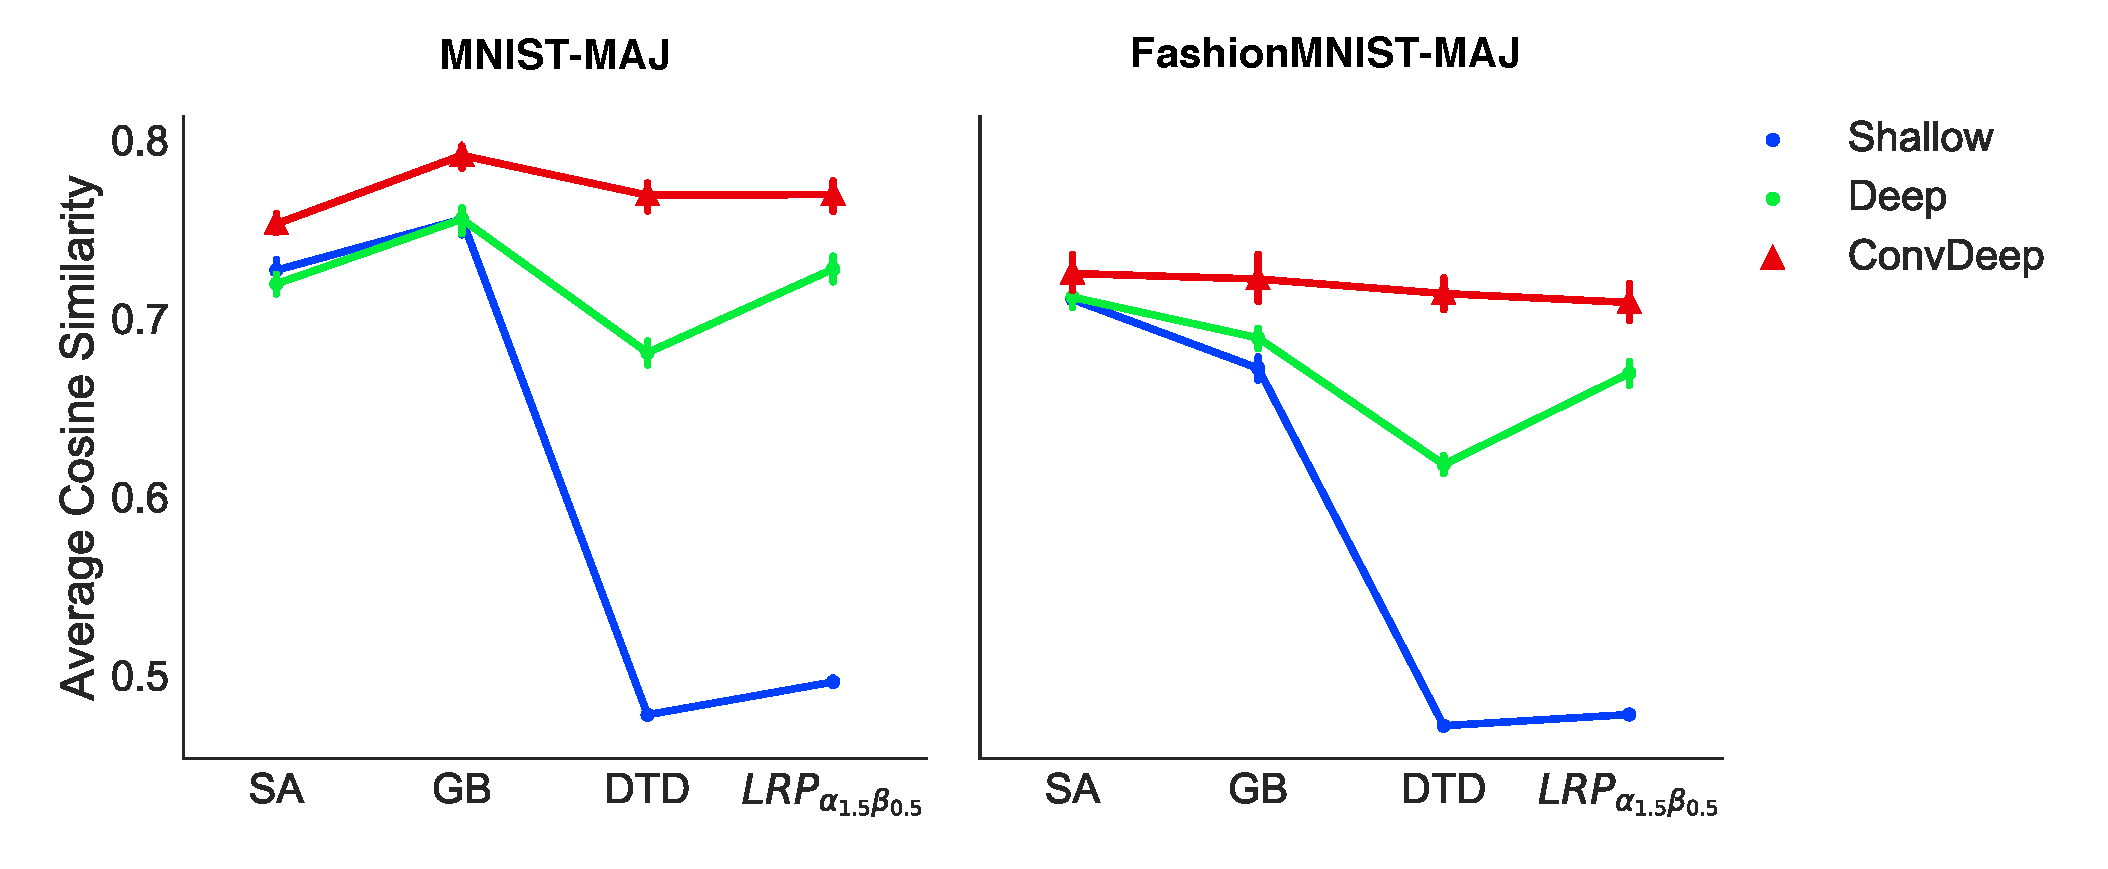
\includegraphics [width=\textwidth]{figures/present_exp1_result_eval}
\end{figure}
\vfill

}


\end{frame}
\begin{frame}{Experiment 2: More Explainable Models}

\only<1> {
\textbf{Motivation:} addressing the improper relevance assignment
\vfill
 \begin{figure}[h]
	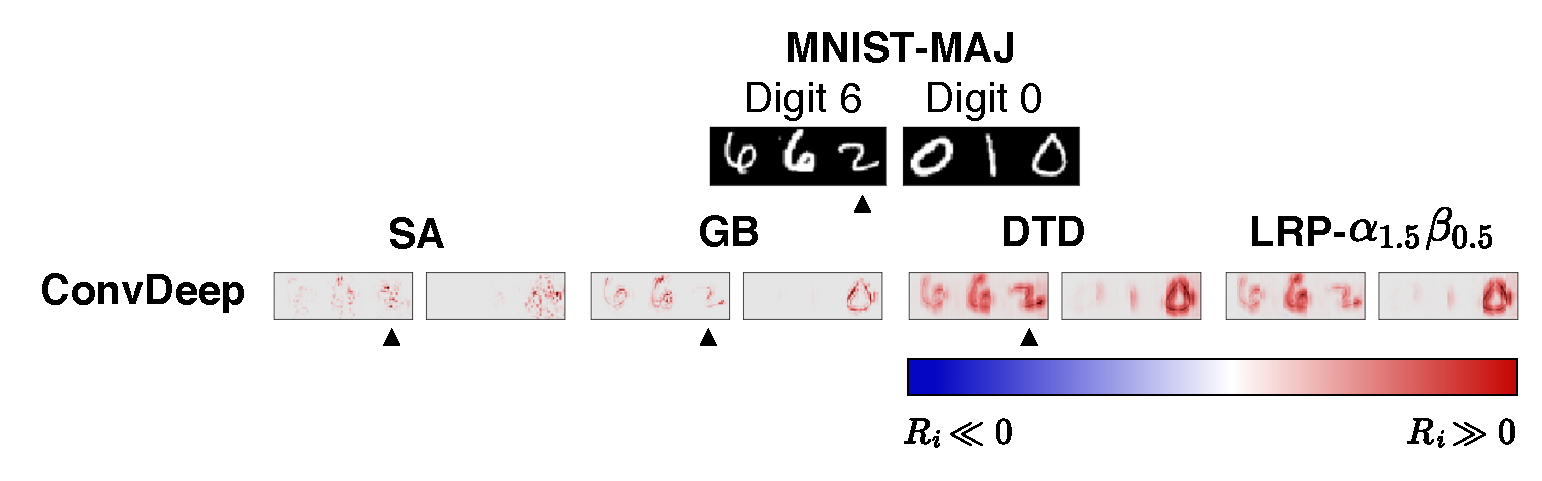
\includegraphics [width=0.8\textwidth]{figures/present_exp2_motivation_only_mnist}
\end{figure}
\vfill

}
\only<2-4>{

\begin{enumerate}

	\item<2->LSTM \citep{HochreiterLongShortTermMemory1997} 

	\only<2>{
				--- Ignore gating neurons during explaining \citep{ArrasExplainingRecurrentNeural2017} \\
				--- Replace tanh by ReLU (R-LSTM) 
		\vfill
		 \begin{figure}[h]
			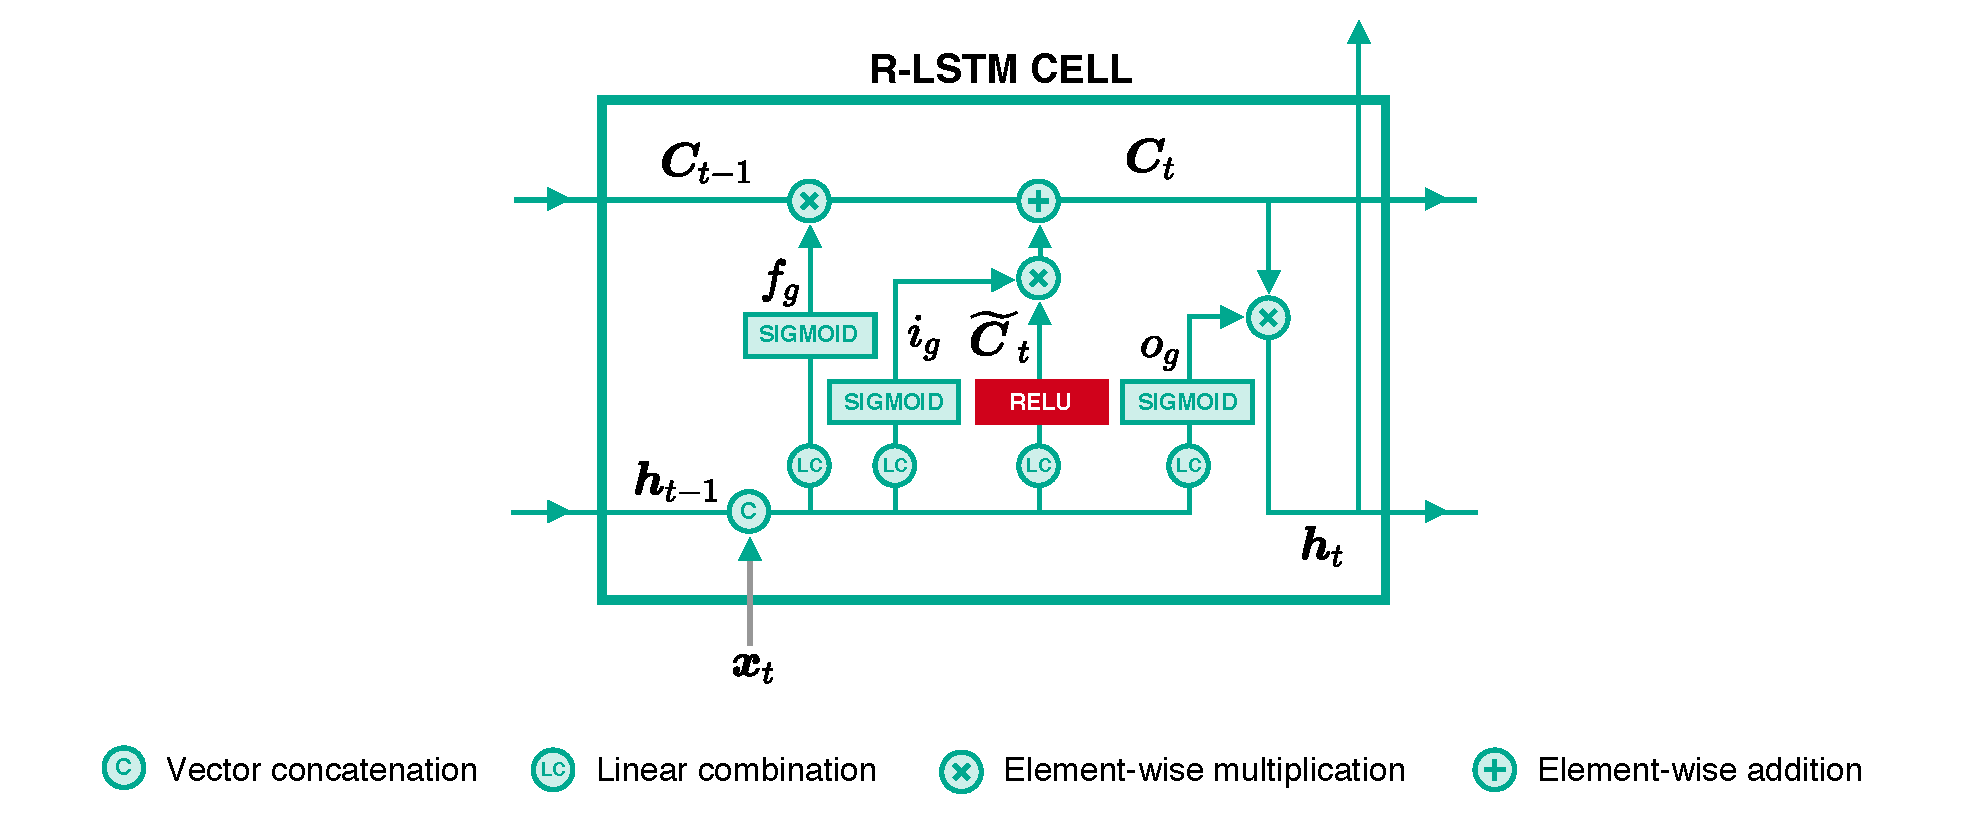
\includegraphics [width=\textwidth]{figures/present_rlstm}
		\end{figure}
		\vfill

	}
	\item<3-> 
	Stationary Dropout (\textit{Variational Recurrent}
		\citep{GalTheoreticallyGroundedApplication2016}) 
		\only<3>{
		\vfill
		 \begin{figure}[h]
			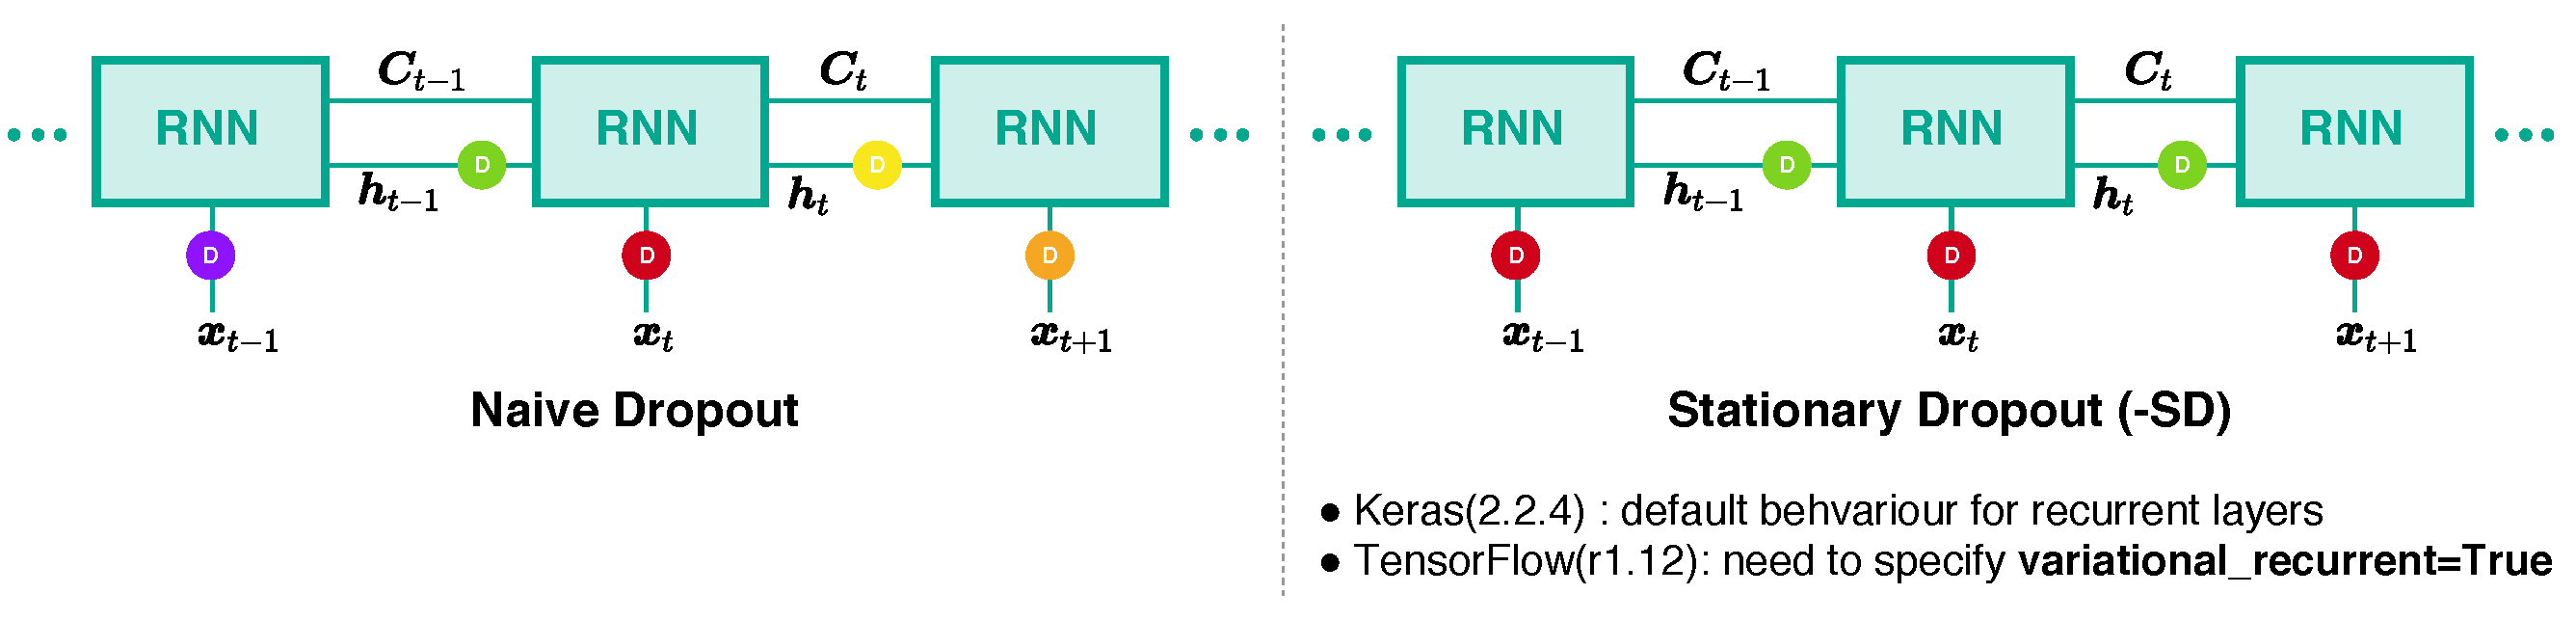
\includegraphics [width=0.9\textwidth]{figures/present_dropout_comparison}
		\end{figure}
		\vfill
		}
		
	\item<4> { Lateral connections for convolutional layers (Conv$^+$)
		\only<4>{
			\vfill
		 \begin{figure}[h]
			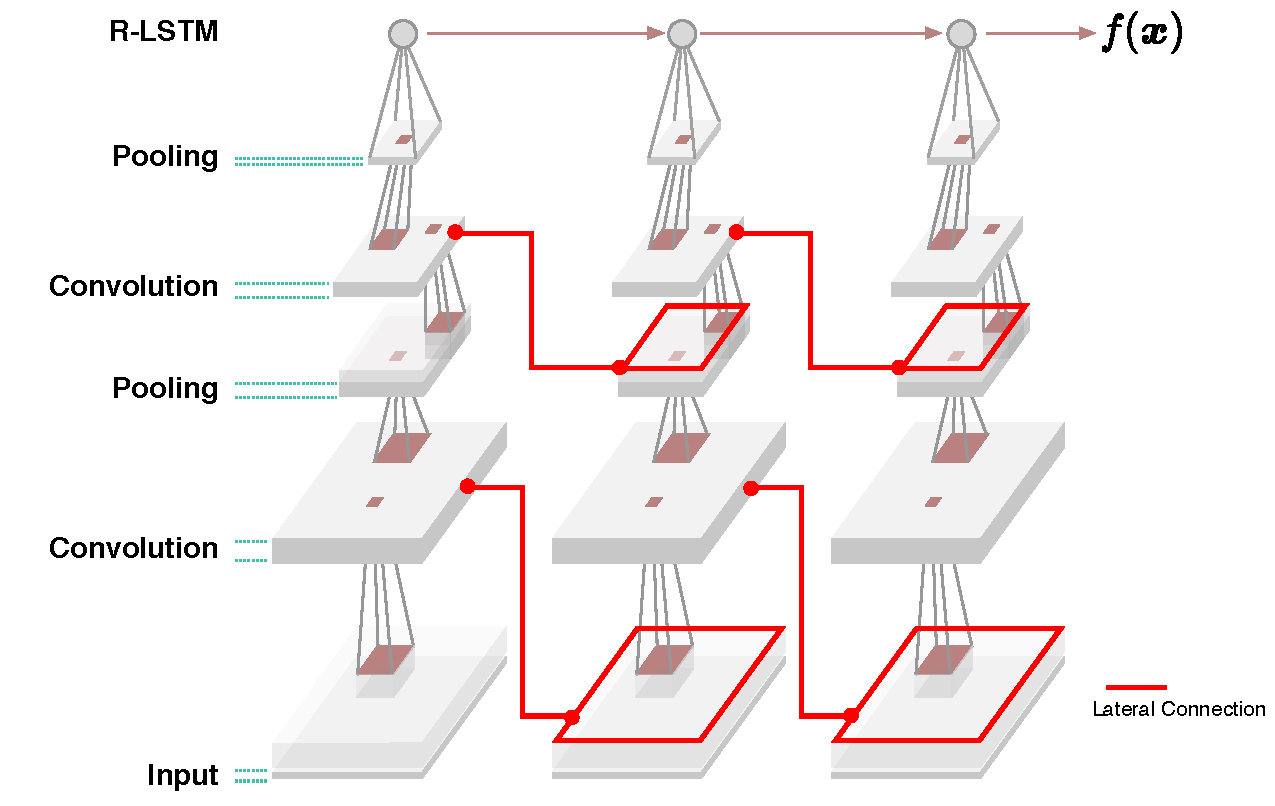
\includegraphics [width=0.6\textwidth]{figures/present_conv_lat_rlstm}
		\end{figure}
		\vfill
		}
		
	}
\end{enumerate}
}

		\only<5>{
		Sample Relevance Heatmaps
		\vfill
		
		 \begin{figure}[h]
			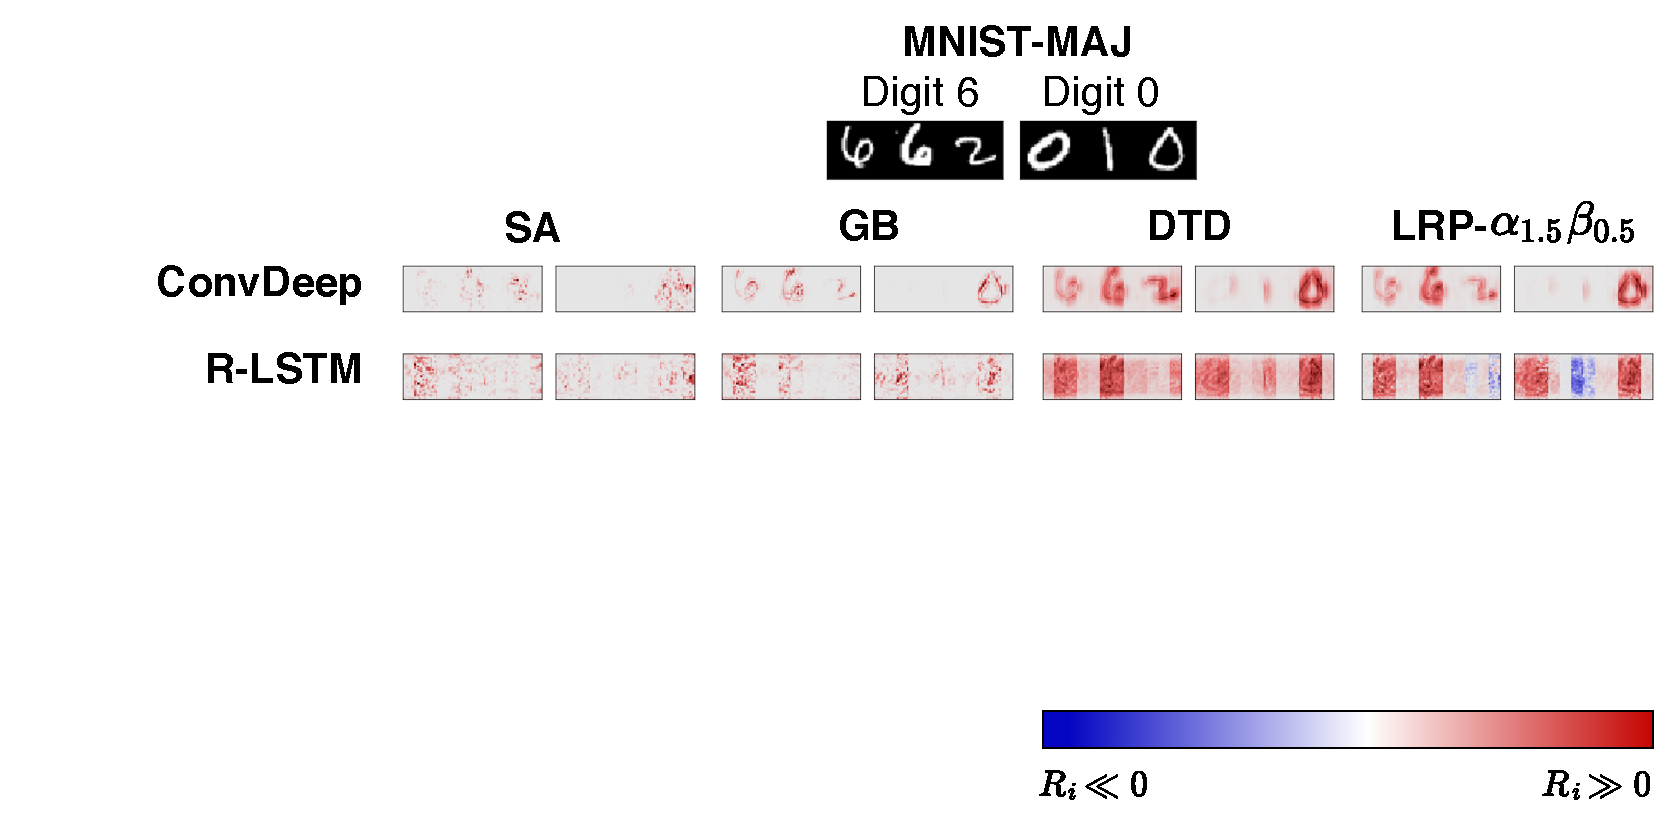
\includegraphics [width=0.8\textwidth]{figures/present_exp2_result_heatmap_1_only_mnist}
		\end{figure}
		
		\vfill
		
		}
		\only<6>{
		Sample Relevance Heatmaps
		\vfill
		
		 \begin{figure}[h]
			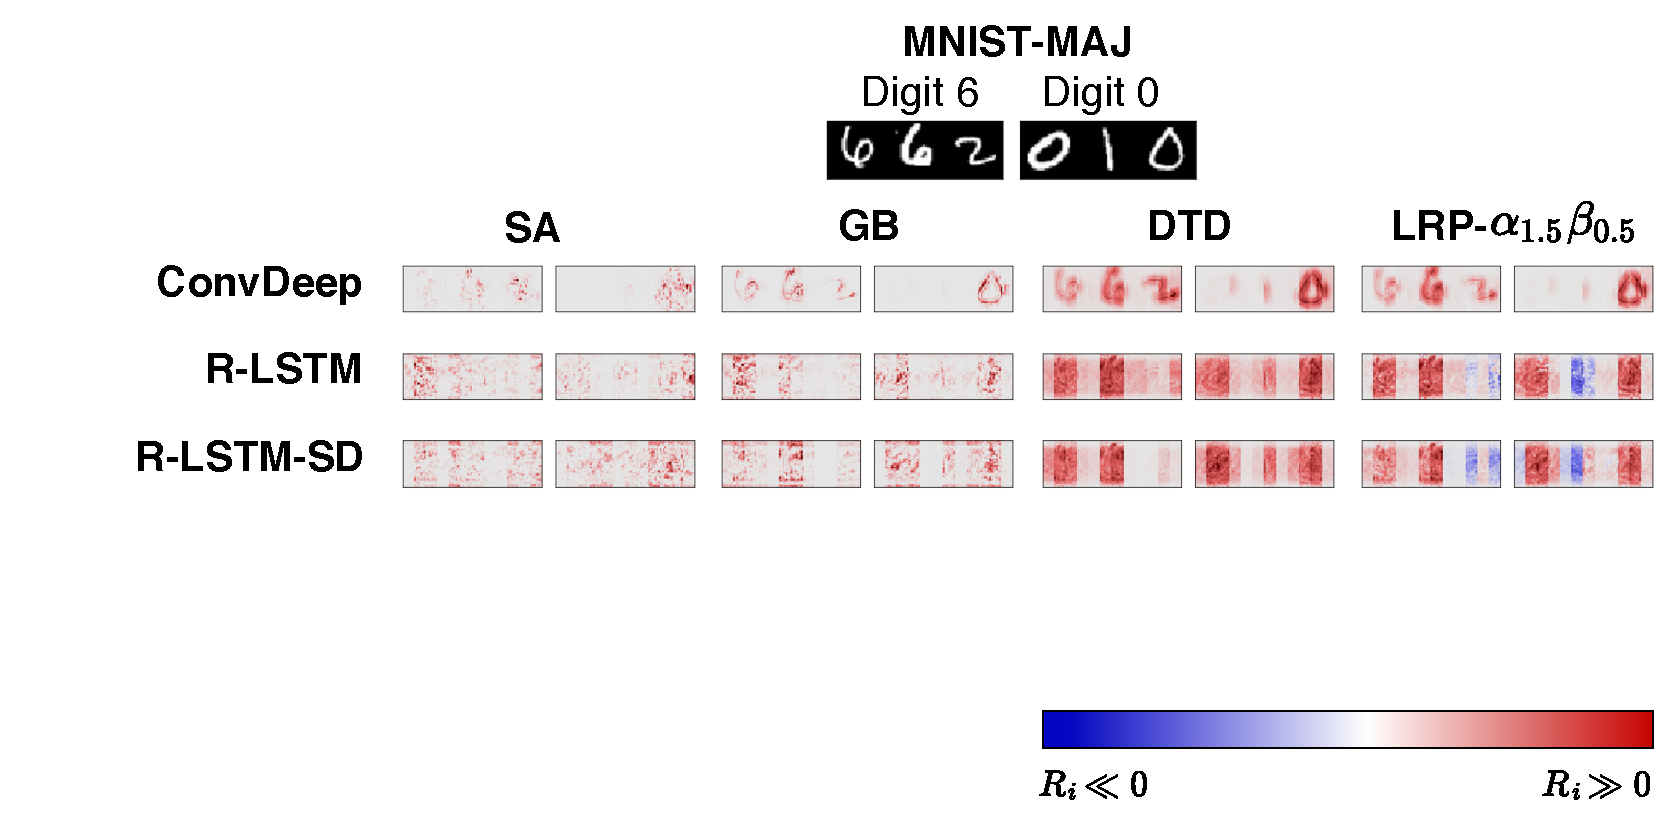
\includegraphics [width=0.8\textwidth]{figures/present_exp2_result_heatmap_2_only_mnist}
		\end{figure}
		
		\vfill
		
		}
		
		\only<7>{
Cosine Similarity Evaluation
\vfill
 \begin{figure}[h]
	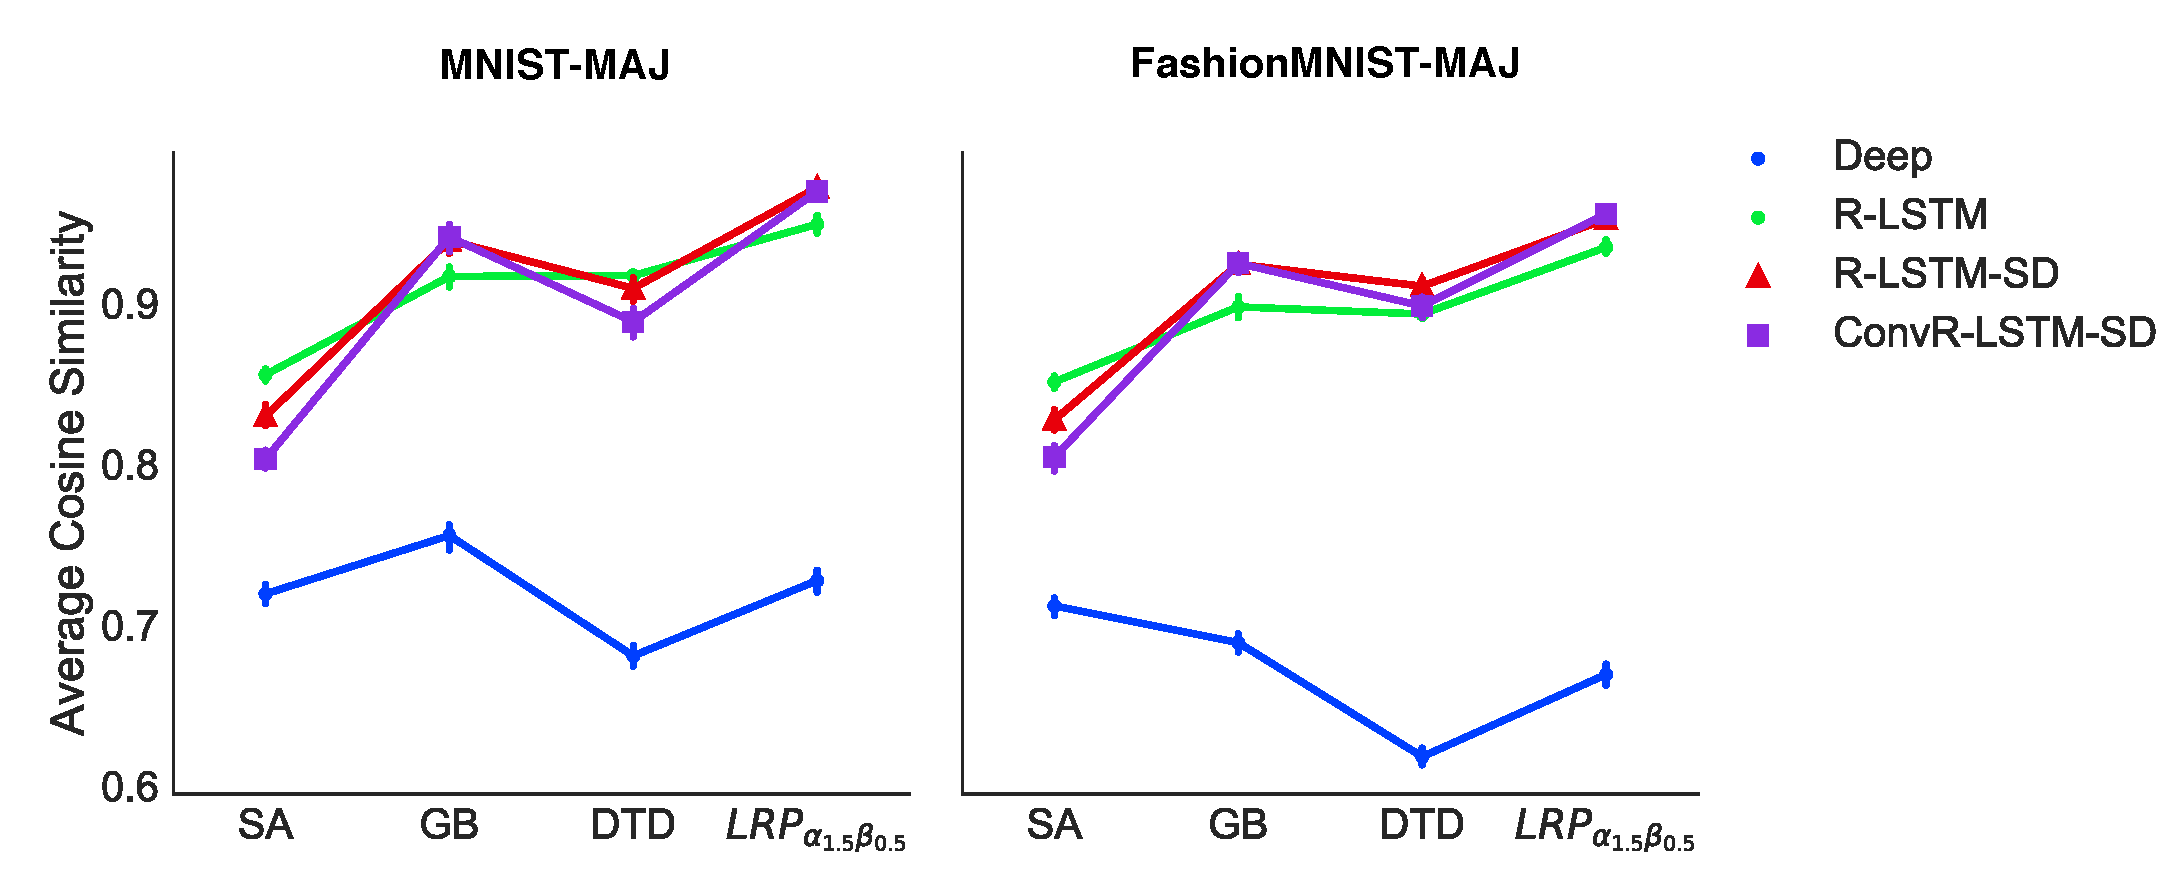
\includegraphics [width=\textwidth]{figures/present_exp2_result_eval}
\end{figure}
\vfill

}
		
		\only<8>{
		Sample Relevance Heatmaps
		\vfill
		
		 \begin{figure}[h]
			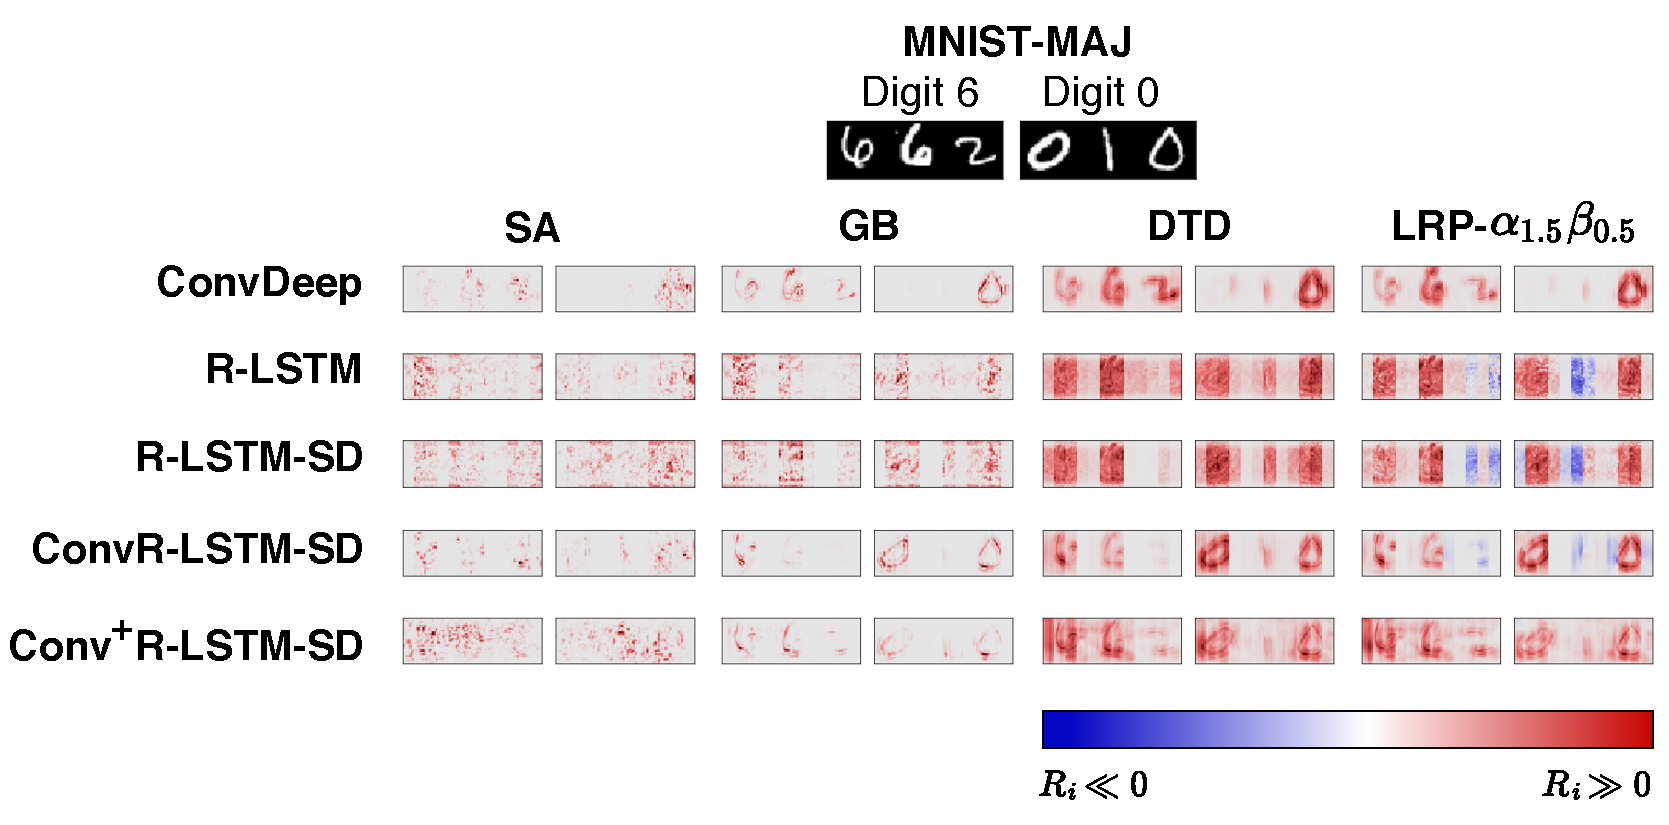
\includegraphics [width=0.8\textwidth]{figures/present_exp2_result_heatmap_3_only_mnist}
		\end{figure}
		
		\vfill
		
		}


\only<9>{
Cosine Similarity Evaluation
\vfill
 \begin{figure}[h]
	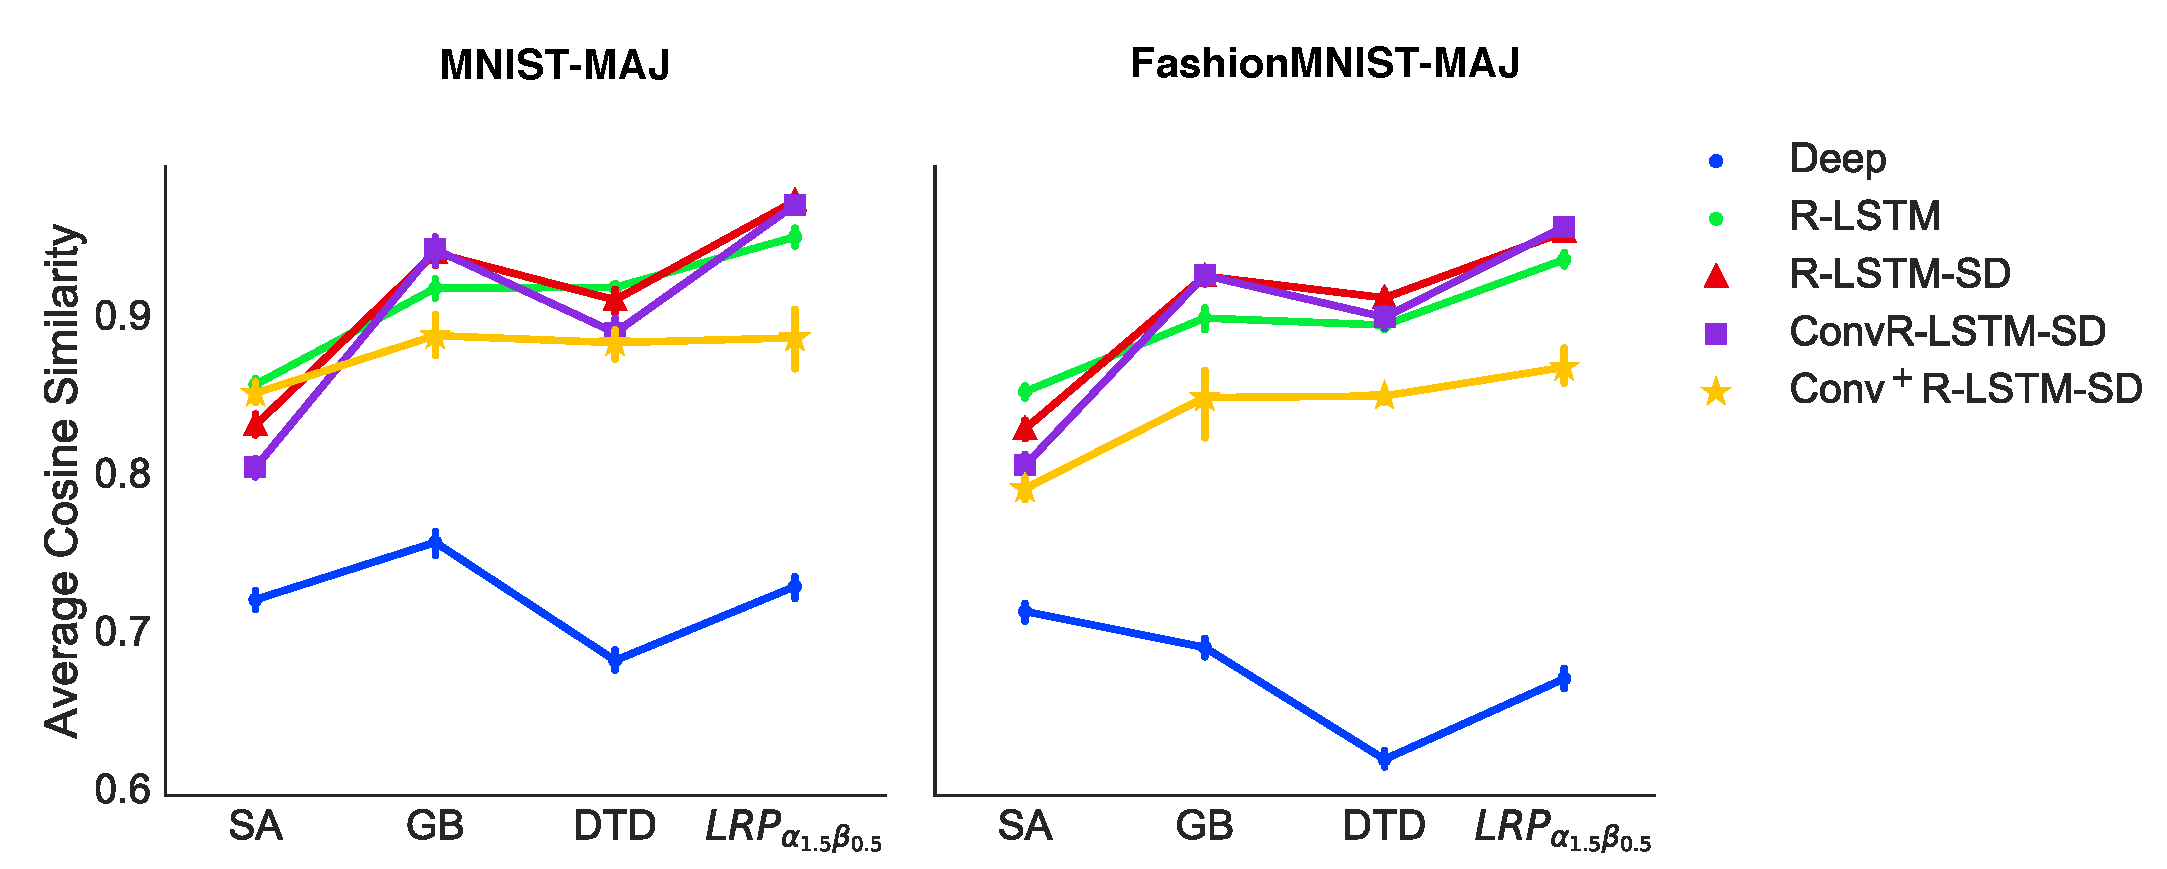
\includegraphics [width=\textwidth]{figures/present_exp2_result_eval_2}
\end{figure}
\vfill

}


\end{frame}


\begin{frame}{Conclusion}

\begin{itemize}
	\item \textbf{Deep and LSTM-type RNNs} have more explainable predictions.
	\item \textbf{Stationary dropout} could improve model's explainability.
	\item Explainability of RNNs should be considered in two aspects:
	 \begin{figure}[h]
	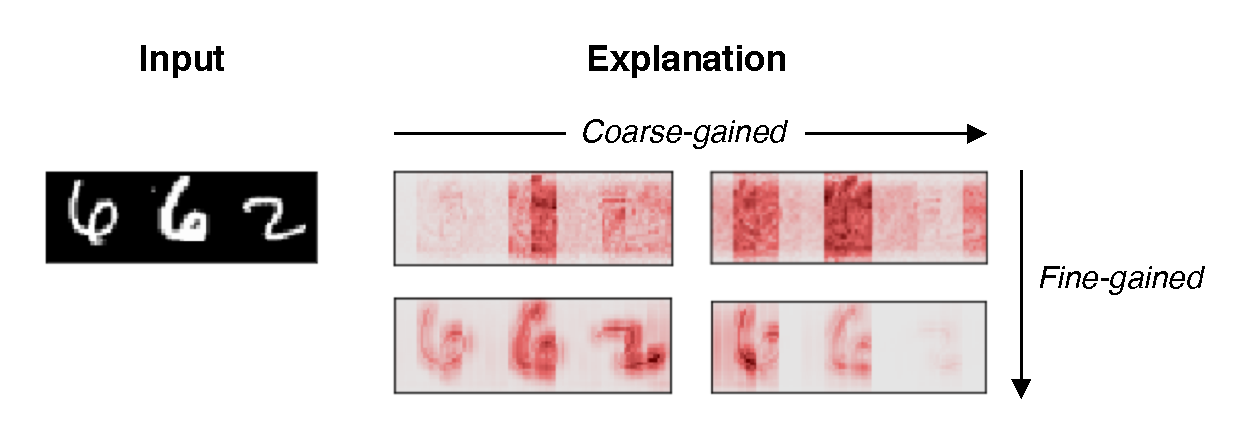
\includegraphics [width=0.65\textwidth]{figures/present_coarse_fine_aspects}
\end{figure}
		\begin{itemize}
			\item \textbf{Coarse-gained}: relevance quantities adequately propagated to relevant steps \\
					--- solution: better recurrent mechanism (i.e. LSTMs)
			\item \textbf{Fine-gained}: soundness of each step's explanation\\
					--- solution: choice of input layers (i.e. convolution and pooling layers for image data)
		\end{itemize}
\end{itemize}
\end{frame}


\begin{frame}{}
\vfill 
\begin{center}
\LARGE \textbf{Q\&A}	
\end{center}

\vfill


\begin{itemize}
	\item[$\blacktriangleright$] Part of this work is in \\
{ \small \vspace{0.2cm}

Rieger, L., Chormai, P., Montavon, G., Hansen, L. K., \& Müller, K. R. (2018). \textbf{Structuring Neural Networks for More Explainable Predictions.} In \textit{Explainable and Interpretable Models in Computer Vision and Machine Learning} (pp. 115-131). Springer, Cham.
} 

	\item[$\blacktriangleright$] Code can be found at \textbf{bit.ly/pat-thesis-repo}.
\end{itemize}


\end{frame}

\begin{frame}
\vfill
 \begin{figure}[h]
 	\frametitle{FashionMNIST Heatmaps}
	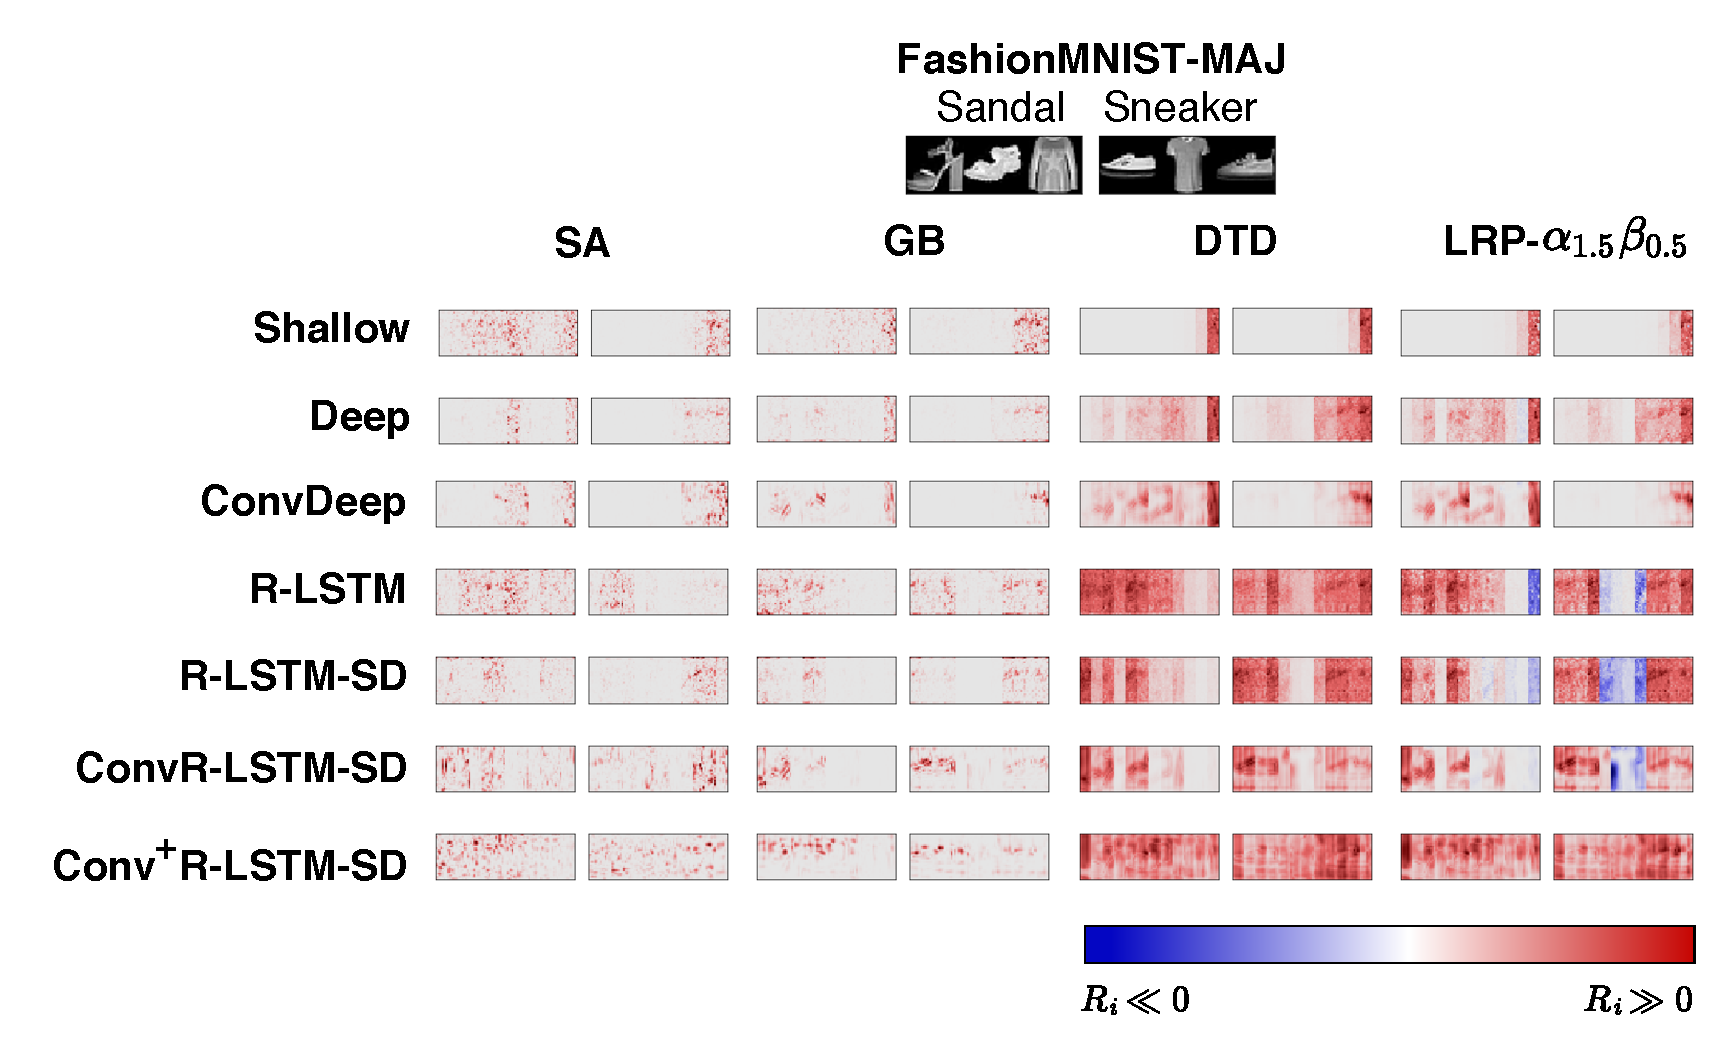
\includegraphics [width=0.8\textwidth]{figures/present_backup_fmnist_heatmaps}
\end{figure}
\vfill
\end{frame}

\begin{frame}
\vfill
 \begin{figure}[h]
 	\frametitle{Model Accuracy}
	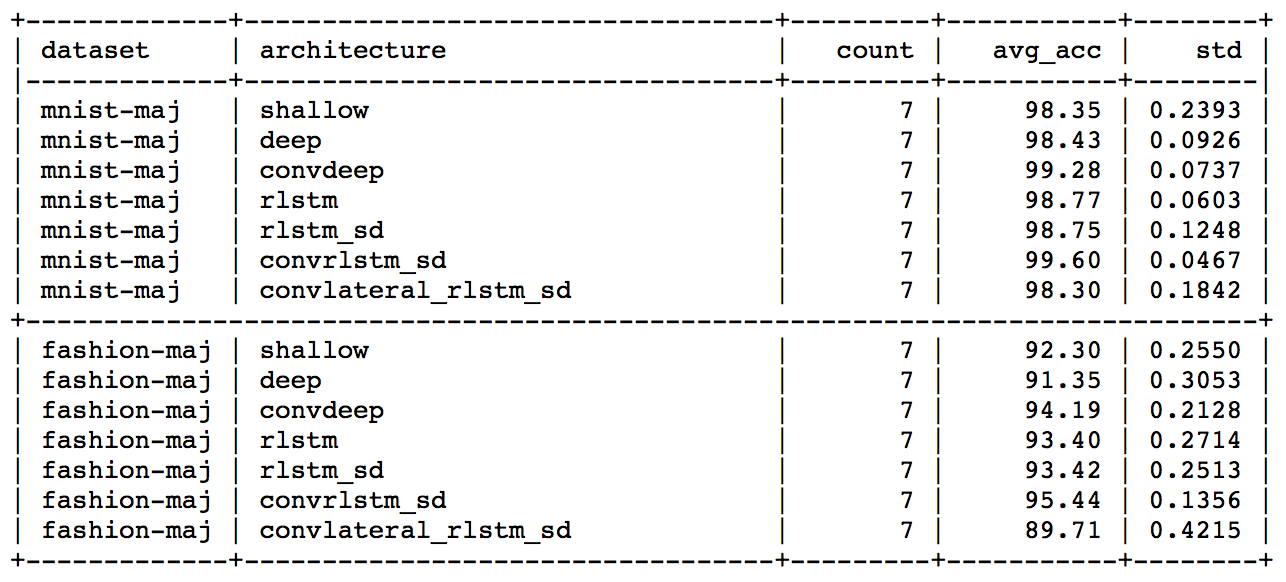
\includegraphics [width=0.8\textwidth]{figures/model_accuracy}
\end{figure}
\vfill
	
\end{frame}


\begin{frame}[allowframebreaks]
        \frametitle{References}
        \bibliographystyle{amsalpha}
        \bibliography{references.bib}
\end{frame}



\end{document}
